%% Copyright 1998 Pepe Kubon
%%
%% `thes-full.tex' --- the example thesis, FULL version, used
%%                     with  the `csthesis' package 
%% Use: latex thes-full to generate the DVI output, then 
%%      bibtex thes-full to generate the bibliography
%%      makeindex thes-full to get the index, and
%%      latex thes-full (2x) 
%%
%% You are allowed to distribute this file together with all files
%% mentioned in READ.ME.
%%
%% You are not allowed to modify its contents.
%%
\documentclass[11pt]{report}
%\documentclass[11pt,twoside]{report}%% for two-sided printing
\usepackage{pdfpages} 
\usepackage{anysize,fancyhdr,graphics}
\usepackage{csthesis}
\usepackage{makeidx}  %%% standard INDEX
\usepackage[titletoc]{appendix}%%Ensure word appendix appears in toc
\usepackage[pagebackref=true,pdfstartview=FitH,bookmarksopen=false,colorlinks,linkcolor=black,citecolor=black]{hyperref} 

\usepackage{mathrsfs}
\usepackage[noend, algo2e, linesnumbered, ruled]{algorithm2e}
\usepackage{epsfig}
\usepackage{epsf}
\usepackage{graphicx}
\usepackage{subfigure}
\usepackage{graphicx,ctable,booktabs}
\usepackage{hyperref}
\usepackage{multirow}
\usepackage{arydshln}
\usepackage{caption}
\usepackage{amsmath}
\usepackage{amsthm}
\usepackage{mathtools}
\usepackage{amssymb}
\usepackage{epsfig}
\usepackage{color}
\usepackage{algorithm,algorithmic}

\renewcommand{\algorithmicrequire}{\textbf{Input:}}
\renewcommand{\algorithmicensure}{\textbf{Output:}}

\usepackage[export]{adjustbox}

\newtheorem{definition}{Definition}[chapter] 
\newtheorem{property}{Property}[chapter] 
\newtheorem{example}{Example}[chapter] 
%\newtheorem{proof}{proof}[chapter]   
%\newtheorem{lemma}{Lemma}[section]  

%\usepackage{enumitem}
%\setlist{nolistsep}
\renewcommand\arraystretch{1.1}
%\renewcommand{\baselinestretch}{0.96}
\newcommand{\nop}[1]{}

\newcommand{\comment}[1]{{\bf [{\color{blue}\sc from Jian:} {\color{red} #1}]}}
\newcommand{\commentXiaoning}[1]{{\bf [{\color{orange}\sc from Xiaoning:} {\color{blue} #1}]}}

\makeatletter
\def\contentsline#1#2#3#4{%
  \ifx\\#4\\%
    \csname l@#1\endcsname{#2}{#3}%
  \else
    \csname l@#1\endcsname{%
      \hyper@linkstart{link}{#4}{#2}\hyper@linkend
    }{%
      % same link destination for the page:
      \hyper@linkstart{link}{#4}{#3}\hyper@linkend
      % link destination is the page itself:
      % \hyperpage{#3}%
    }%
  \fi
} \makeatother


\makeindex  

%%% The following code demonstrates the ``other list'' facility. A new
%%% command \otherlist is defined for the List of Programs. Programs
%%% are defined as floating environments of type 3 (1 is used for figures,
%%% 2 for tables) and the information about them is stored in an
%%% auxiliary file with .lop extension. You can use this method to
%%% define several types of ``other lists,'' but in that case you'll
%%% need to add appropriate code to \lists in the csthesis.sty
%%% package.
%%% Note: It's better to move this code into your own mythesis.sty
%%% package. If you do that, you should get rid of the \makeatletter,
%%% \makeatother commands.
%\makeatletter
%\newcommand\otherlist{%
%    \addcontentsline{toc}{chapter}{\otherlistname}
%    \if@twocolumn
 %     \@restonecoltrue\onecolumn
%    \else
%      \@restonecolfalse
%    \fi
%    \chapter*{\otherlistname
%      \@mkboth{\MakeUppercase\otherlistname}%
%              {\MakeUppercase\otherlistname}}%
%    \@starttoc{lop}%
%    \if@restonecol\twocolumn\fi
%    }
%\newcommand*\l@program{\@dottedtocline{1}{1.5em}{2.3em}}
%\newcommand\otherlistname{List of Programs}
%\newcommand\programname{Program}
%\newcounter{program}[chapter]
%\renewcommand\theprogram{\thechapter.\@arabic\c@program}
%\def\fps@program{tbp}
%\def\ftype@program{3}
%\def\ext@program{lop}
%\def\fnum@program{\programname~\theprogram}
%\newenvironment{program}
%               {\@float{program}}
%               {\end@float}
%\newenvironment{program*}
%               {\@dblfloat{program}}
%               {\end@dblfloat}
%\makeatother
%%% end of ``other list'' code

\begin{document}
\setlength{\pdfpagewidth}{8.5in}
\setlength{\pdfpageheight}{11in}
%%% set switches
%\contentspagefalse  
\figurespagetrue
\tablespagetrue
\dedicationpagetrue
\quotationpagetrue
%\otherlistpagetrue

%%% front matter 
%% Copyright 1998 Pepe Kubon
%%
%% `titapp.tex' --- title and approval for thes-full.tex, thes-short-tex from
%%                  the `csthesis' bundle
%%
%% You are allowed to distribute this file together with all files
%% mentioned in READ.ME.
%%
%% You are not allowed to modify its contents.
%%

%%%%%%%%%%%%%%%%%%%%%%%%%%%%%%%%%%%%%%%%%%%%%
%
%   Title and approval pages
%
%%%%%%%%%%%%%%%%%%%%%%%%%%%%%%%%%%%%%%%%%%%%%

%%% title page

\title{Individual Skyline Subspace on User Annotated Tags}
\author{Jiaxing Liang}
\qualification{B.Sc., Simon Fraser University, 2013}
\qualification{B.Eng., Zhejiang University, 2013}
\submitdate{Spring 2015}
\copyrightyear{2015}

%%% approval page


\chair{Dr.~Ha Ha,\\
	Associate Professor, } 
\signatory{Dr.~Jian Pei,\\
        Professor, 
%        Computing Science,\\
%       %Simon Fraser University\\ 
       Senior Supervisor}
\signatory{Dr.~Martin Ester,\\
        Professor, 
%        Computing Science,\\
%       %Simon Fraser University\\ 
       Supervisor}
       
\signatory{Dr.~Ha Ha,\\
       Associate Professor,
       %Computing Science,
%       %Simon Fraser University\\ 
       Internal Examiner}


%%% generating title and approval pages 
\beforepreface

 %% title, approval

%% Partial Copyright License (PCL)
%% Please check the library online regulations & Forms, http://www.lib.sfu.ca/thesis
\newpage 			
\addcontentsline{toc}{chapter}{Partial Copyright License}
\mbox{}
\makeatletter
\AddToShipoutPictureBG*{
            \setlength{\@tempdimc}{.06\paperheight}
            \setlength{\unitlength}{1pt}
           \put(\strip@pt\@tempdimb,\strip@pt\@tempdimc){
	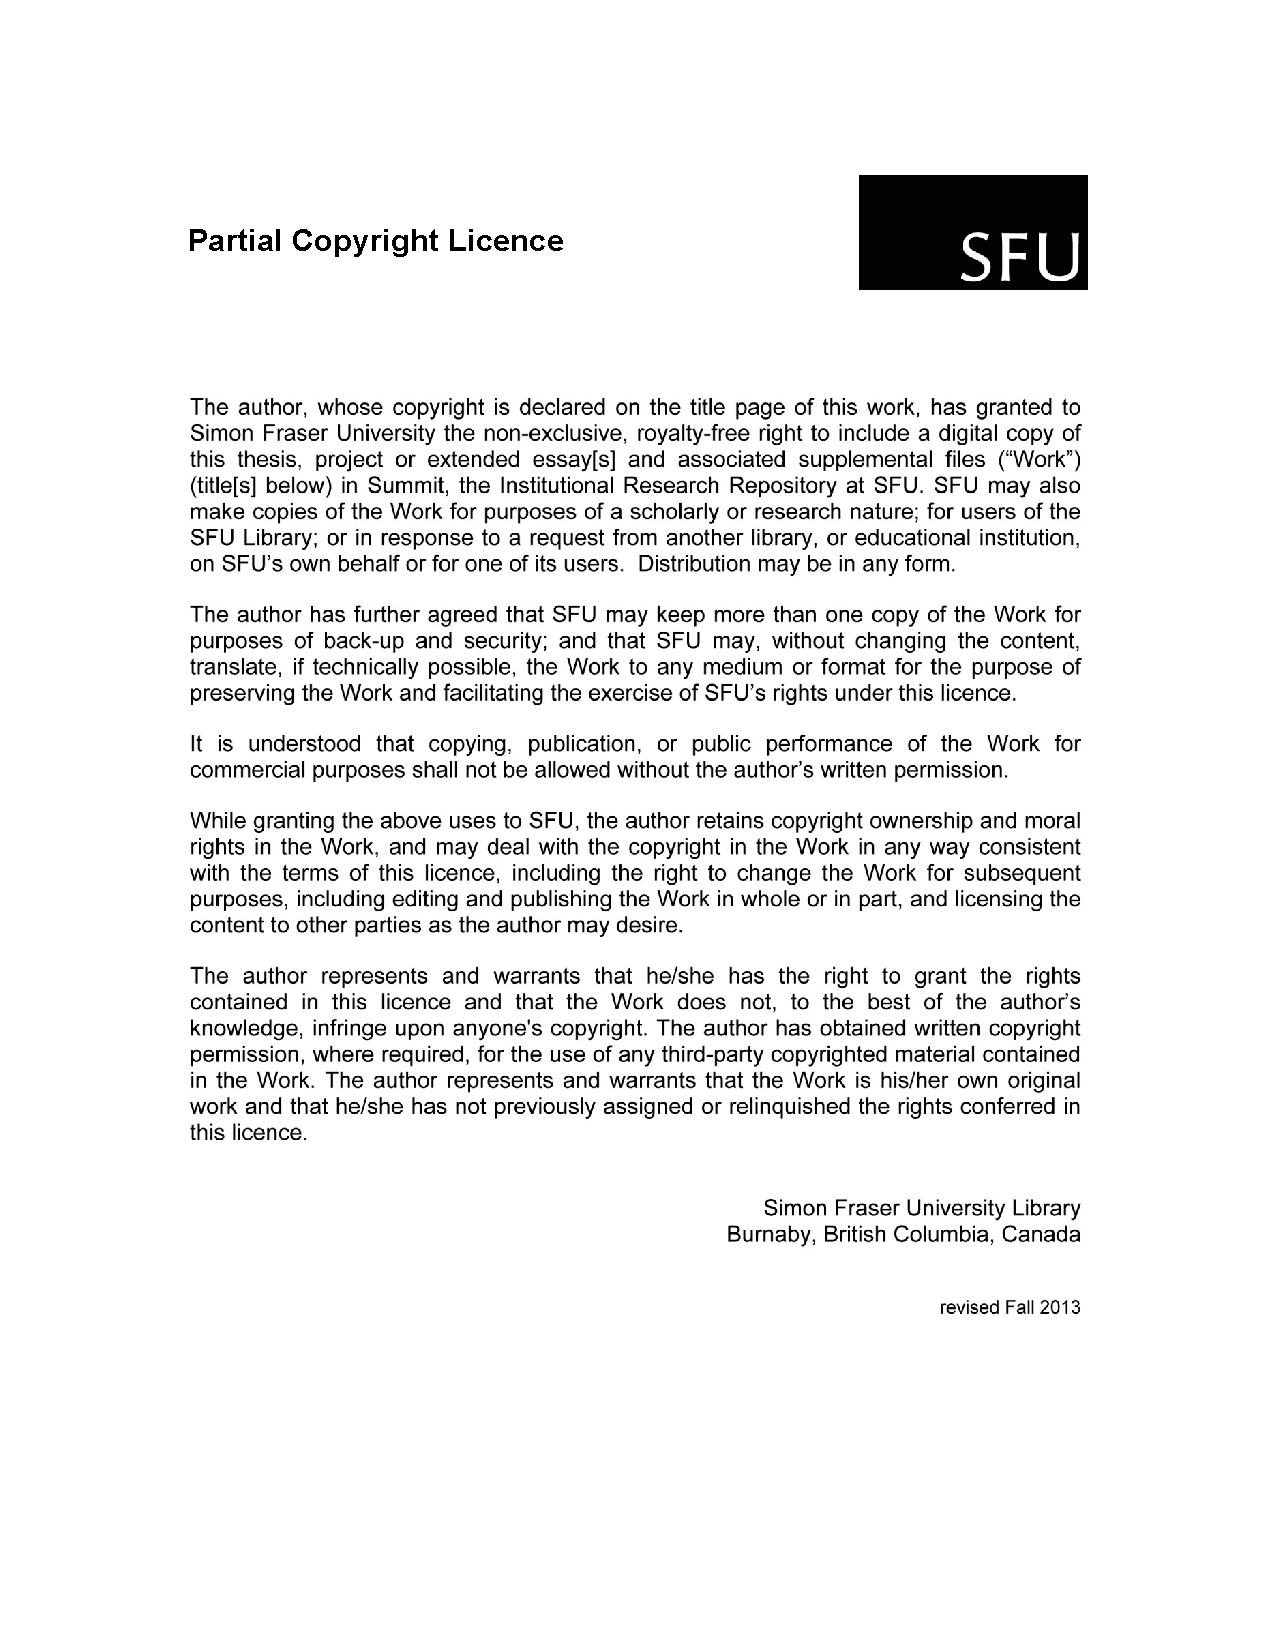
\includegraphics{PCL_Declaration.pdf}
	} 
} 
\makeatother
\newpage

% !TEX root = ../topk_thesis.tex
%% Copyright 1998 Pepe Kubon
%%
%% `abstract.tex' --- abstract for thes-full.tex, thes-short-tex from
%%                    the `csthesis' bundle
%%
%% You are allowed to distribute this file together with all files
%% mentioned in READ.ME.
%%
%% You are not allowed to modify its contents.
%%

%%%%%%%%%%%%%%%%%%%%%%%%%%%%%%%%%%%%%%%%%%%%%%%%%
%
%       Abstract    
%
%%%%%%%%%%%%%%%%%%%%%%%%%%%%%%%%%%%%%%%%%%%%%%%%

\prefacesection{Abstract}

Skyline computation is important in applications that involve multi-criteria decision making. In this thesis, we consider the problem: given a query point, the subspaces where the query point is in the subspace skyline. Although efficient algorithms for subspace skyline computation have developed in many existing studies, finding skyline subspaces for one certain query point is still an open problem. We develop an algorithm based on bottom-up set enumeration to compute the skyline to compute the skyline subspace efficiently. We formulate the problem of identify the uniqueness of a given vertex to skyline subspace queries problem on graph and proposed effective pruning methods to tackle this problem. We further conduct experiments on both real world datasets and synthetic datasets to verify the efficiency of our model.










 %% abstract
%% Copyright 1998 Pepe Kubon
%%
%% `dedquot.tex' --- dedication and quotation for thes-full.tex from
%%                   the `csthesis' bundle
%%
%% You are allowed to distribute this file together with all files
%% mentioned in READ.ME.
%%
%% You are not allowed to modify its contents.
%%

%%%%%%%%%%%%%%%%%%%%%%%%%%%%%%%%%%%%%%%%%%%%%
%
%   Dedication/Quotation pages
%
%%%%%%%%%%%%%%%%%%%%%%%%%%%%%%%%%%%%%%%%%%%%%

\dedication{To my parents.}
\thesquot{%
``You will recognize your own path when you come upon it, because you \\will suddenly have all the energy and imagination you will ever need.''\\[5pt]%
--- \textsc{Jerry Gillies}, (1940- )%
}

%%% generate pages
\dedicquotation
 %% dedication and quotation, if any 
%% Copyright 1998 Pepe Kubon
%%
%% `ack.tex' --- aknowledgments for thes-full.tex, thes-short-tex from
%%               the `csthesis' bundle
%%
%% You are allowed to distribute this file together with all files
%% mentioned in READ.ME.
%%
%% You are not allowed to modify its contents.
%%

%%%%%%%%%%%%%%%%%%%%%%%%%%%%%%%%%%%%%%%%%%%
%
%       Acknowledgment 
%
%%%%%%%%%%%%%%%%%%%%%%%%%%%%%%%%%%%%%%%%%%

\prefacesection{Acknowledgments}
I would like to express my deepest gratitude to my senior supervisor, Dr.~Jian Pei, for his great patience, warm encouragement and continuous support throughout my Master's studies. His wisdom and passion in research has influenced and inspired me a lot, which gave me confidence and interest in accomplishing this thesis. 

I would like to thank Dr.~Martin Ester for being my supervisor and giving me helpful suggestions on my thesis. I also thank Dr.~Ha Ha and Dr.~Ha Ha for serving in my examining committee.  

I am also very grateful to my lab mates for their kind help. A special thank goes to Dr.~Huaizhong Lin, Dr.~Aihua Wu, Dr.~Fuyuan Cao, Dr.~Kui Yu,  Dr.~Dongwan Choi, Guanting Tang, Xiao Meng, Juhua Hu, Chuancong Gao, Yu Yang, Xiangbo Mao, Xuefei Li, Lumin Zhang, Xiang Wang, Xiaoning Xu, Yu Tao, Lin Liu, Li Xiong, Beier Lu, Zicong Cun, and Xiaojian Wang.

Moreover, my sincerest gratitude goes to my parents for their endless love and support through all these years.
 %%  acknowledgments

%%%  generate contents, lists of figures, etc.
\lists

%% preface (foreword), if any
% %% Copyright 1998 Pepe Kubon
%%
%% `preface.tex' --- preface for thes-full.tex from
%%                   the `csthesis' bundle
%%
%% You are allowed to distribute this file together with all files
%% mentioned in READ.ME.
%%
%% You are not allowed to modify its contents.
%%

%%%%%%%%%%%%%%%%%%%%%%%%%%%%%%%%%%%%%%%%%%%%%%%%%
%
%       Preface 
%
%%%%%%%%%%%%%%%%%%%%%%%%%%%%%%%%%%%%%%%%%%%%%%%%

\prefacesection{Preface}
Here go all the interesting reasons why you decided to write this thesis.

 

%%% prepare main section
\beforetext

%%% main matter
% !TEX root = ../topk_thesis.tex
%% Copyright 1998 Pepe Kubon
%%
%% `one.tex' --- 1st chapter for thes-full.tex, thes-short-tex from
%%                the `csthesis' bundle
%%
%% You are allowed to distribute this file together with all files
%% mentioned in READ.ME.
%%
%% You are not allowed to modify its contents.
%%

%%%%%%%%%%%%%%%%%%%%%%%%%%%%%%%%%%%%%%%%%%%%%%%%%
%
%       Chapter 1 
%
%%%%%%%%%%%%%%%%%%%%%%%%%%%%%%%%%%%%%%%%%%%%%%%%

\chapter{Introduction}

In this chapter, we first introduce the basic idea of skyline subspace problem and several interesting applications that motivate the problem, which will be studied in this thesis. Then, we will summarize the major contributions and describe the structure of the thesis.

\section{Motivations}
The skyline operator is an important research topic for multi-criteria decision making applications.

One classical example of skyline queries is searching for hotels that are cheap and close to the beach~\cite{borzsony2001skyline}. We assume that each hotel has two attributes: the price and the distance from the hotel to the beach.
Suppose there is Hotel A and Hotel B and the price of Hotel A is lower than the price of Hotel B, and the distance from Hotel A to the beach is also shorter than the distance from Hotel B to beach.
Then Hotel A dominates Hotel B.
We call those hotels that are not dominated by others in terms of price and distance to the beach skyline hotels. 
There are many recent studies on efficient methods for skyline computation, subspace skyline analysis and skyline computation in different scenarios. We will review the related work on Chapter~\ref{ch:related-work}.

However, all the previous studies are about the skyline computation. The questions about computing the subspaces of a query point with respect to skyline remain open.

\begin{figure}[H]
\centering
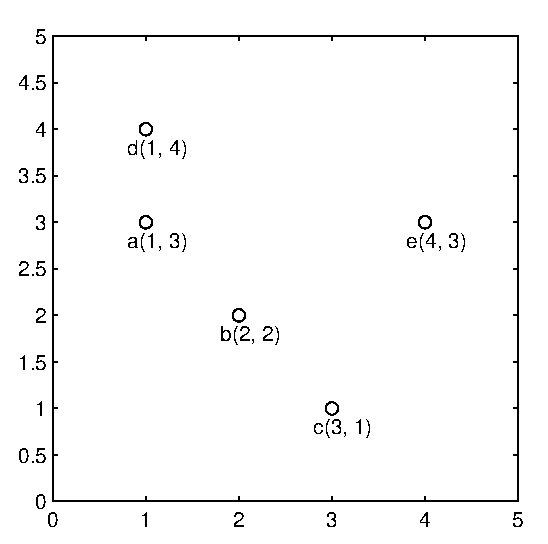
\includegraphics[width=0.5\textwidth]{figs/intro_xy.eps}
\caption{An example of data points on full space $(X, Y)$}
\label{fig:intro_xy}
\end{figure}

\begin{figure}[H]
\centering
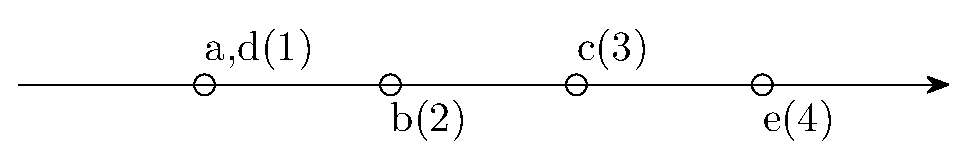
\includegraphics[width=0.5\textwidth]{figs/intro_x.eps}
\caption{The projection of data points on subspace $X$}
\label{fig:intro_x}
\end{figure}

\begin{figure}[H]
\centering
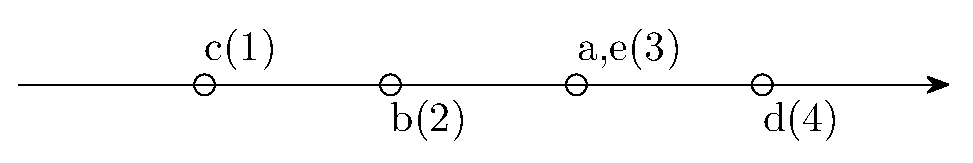
\includegraphics[width=0.5\textwidth]{figs/intro_y.eps}
\caption{The projection of data points on subspace $Y$}
\label{fig:intro_y}
\end{figure}

\begin{example} 
\label{exp:xy:points}
Consider a set of $5$ data points in 2-d space $(X, Y)$ as shown in Figure~\ref{fig:intro_xy}. The points $a$, $b$ and $c$ are skyline points in space $(X, Y)$ since each of them is not dominated by any other points.
\end{example}

In Figure~\ref{fig:intro_x} and Figure~\ref{fig:intro_y}, we also plot the projections of the data points on dimensions $X$ and $Y$, respectively. In our thesis, we are only interested in the non-trivial subspaces that are non-empty. In Example~\ref{exp:xy:points}, subspace $X$ and subspace $Y$ are two non-empty subspaces that we are interested in. In subspace $X$, the projections of the point $a$ and $d$ have the same value. Both of them are subspace skyline points of subspace $X$. In subspace $Y$, the projection of point $c$ is also a skyline point.

From Figure~\ref{fig:intro_xy}, we can see that point $a$, point $b$ and point $c$ are skyline points in the full space $(X, Y)$. However, there are differences among them if we look at them in different projections. Point $a$ is a subspace skyline point in subspace $X$. Point $c$ is a subspace skyline point in subspace $Y$. Although $b$ is also skyline point in the full space $(X, Y)$, it is not a skyline point in projection $X$ or projection $Y$.

Taking the value $1$ on subspace $Y$ is sufficient for $c$ to be a skyline point in the full space $(X, Y)$. No other points are able to dominate $c$ because $c$ is the only point with the minimal value $1$ on subspace $Y$. While taking the value $1$ on subspace $X$ is not sufficient for $a$ to be a skyline point in full space, because $d$ also has the same minimal value $1$ on subspace $X$. Point $b$ does not have minimal value on subspace $X$ or subspace $Y$.

Point $d$ and $e$ are still subtly different although neither of them is a skyline object in full space $(X, Y)$. With the same minimal value $1$ as point $a$ on subspace $X$, point $d$ is a skyline points in subspace $X$. Point $e$ is not a skyline point in full space $(X, Y)$ or any subspaces of $(X, Y)$.

In our thesis, we are interested in finding all the minimal subspace projections such that a query point is a skyline point on those projections. We call these projections \emph{skyline subspaces} of the query point.

\emph{Why are we interested about the skyline subspaces of the query points?} The information of skyline subspace helps us understand the data better. In Section~\ref{ch:exp:graph}, we analyze a real dataset of DBLP citation network. We take the distances from all authors to a conference as a dimension. Consider all conferences as the full space, we want to compute the subspaces on which the query author point is a skyline point. By computing those subspaces, we are able to know what distinguishes an author from its peers in terms of research topics and academic connections of that author. For example, Dr. Stephan Schulz publishes papers or connects with other authors who publish papers in the computing science conferences \emph{ENTCS}, \emph{J. Symb. Log.}, \emph{FLAIRS} and \emph{ACM Trans. Graph.}. Dr. Stephan Schulz is a skyline points in terms of connections and publications in these four conferences and we claim that he has a good reputations in computer science. We are interested in the subsets of these conferences that make him distinguished with others. After computing the skyline subspaces of Dr. Stephan Schulz in the DBLP citation network, we find the distances from Stephan to conferences \emph{ENTCS} and \emph{ACM Trans. Graph.} are $2$ and $1$ respectively, which makes him a skyline point among all the researchers. In Section~\ref{ch:exp:spatial}, we analyze the Yelp academic dataset. Given a query business spot, taking the Euclidean distances between the business spots and the business categories (restaurant, coffee shop, etc.) as criteria, we are interested in finding the sets of business categories that makes the business spot special.

Computing the skyline points of all the subspaces~\cite{pei2005catching, yuan2005efficient} is costly when users are only interested in finding subspaces of a certain the query points. In this thesis, we are focusing on skyline subspaces of one query point but not the whole dataset. The skyline subspace queries is also known as \emph{skyline membership queries} mentioned in \cite{pei2005catching} but the problem of answering \emph{skyline membership queries} efficiently had not been solved.

\section{Contributions}
The original skyline operator problems have been studied in~\cite{borzsony2001skyline, chomicki2003skyline} and subspace skyline problems have been studied in~\cite{pei2005catching, yuan2005efficient}. In this thesis, our goal is to find the subspaces where the query point is in the subspace skylines. By tackling this problem, we make the following contributions.

\begin{itemize}
\item We develop an algorithm framework to answer the \emph{skyline subspace query}, finding the subspaces where a query point is in the subspace skyline. We present a bottom-up algorithm based on set enumeration and dominant candidate sets intersection to solve the problem.

\item We apply skyline subspace query on two specific applications: Computing skyline subspaces on graph and computing the skyline subspaces on Euclidean space. We develop effective pruning algorithms to reduce the unnecessary computation.

\item A performance study using both synthetic and real data sets is conducted to evaluate our approach. For the skyline subspace problem on the graph, we run our algorithm on DBLP citation network to test its efficiency and scalability. For the spatial skyline subspace problem, we run our algorithm on the YELP academic dataset.
\end{itemize}
  

\section{Organization of the Thesis}
The rest of the thesis is organized as follows. In Chapter~\ref{ch:related-work}, we review the related work of skyline queries. We then formulate our \emph{skyline subspace} problem in Chapter~\ref{ch:prob-def}. In Chapter~\ref{ch:graph}, we propose the basic framework of our algorithm and the pruning method on \emph{skyline subspace queries on graph}.  In Chapter~\ref{ch:spatial}, we present our algorithm of \emph{spatial skyline subspace queries}.  We report our experimental results in Chapter~\ref{ch:exp}, and conclude the thesis in Chapter~\ref{ch:con}.










 
%% Copyright 1998 Pepe Kubon
%%
%% `two.tex' --- 2nd chapter for thes-full.tex, thes-short-tex from
%%               the `csthesis' bundle
%%
%% You are allowed to distribute this file together with all files
%% mentioned in READ.ME.
%%Discuss the reality where queries are not randomly generated.
%% You are not allowed to modify its contents.
%%

%%%%%%%%%%%%%%%%%%%%%%%%%%%%%%%%%%%%%%%%%%%%%%%%%
%
%     Chapter 2   
%
%%%%%%%%%%%%%%%%%%%%%%%%%%%%%%%%%%%%%%%%%%%%%%%%

\chapter{Related Work}
\label{ch:related-work}

Our problem of \emph{skyline subspace query} is mainly related to the existing work on general skyline query, subspace skyline computation and skyline query with specific constrain which are reviewed in Section~\ref{sec:rel:general}, Section~\ref{sec:rel:subspace} and Section~\ref{sec:rel:constrain}, respectively.

\section{General Skyline Query}
\label{sec:rel:general}
The general skyline problem is to find all the points that are not dominated by any other points.
There is a number of studies of skyline in Data Mining area. The problem of finding the maxima (skyline) of a set of vectors is first investigated in~\cite{kung1975finding} where an $O(n\log ^{d-2}n)$ algorithm for dimension $d\geq 4$ and an $O(n\log n)$ time algorithm for dimension $d = 2, 3$ are proposed. The algorithm in~\cite{kung1975finding} is based on the divide and conquer principle. To integrate the skyline operator into database, Borzsony et al.~\cite{borzsony2001skyline} proposed the Block-nested-loops Algorithm (BNL) and Divide and Conquer Algorithm (DC) to compute the skyline queries. BNL essentially maintain a window of incomparable and compare each object in the database with the objects in the window and outputs the skyline at the end of the iteration. DC divides the dataset into several partitions and each partition can fit in memory. The skylines in all partitions are computed individually in main memory, and then merged to produce the final skyline objects. 
The sort-first-skyline (SFS)~\cite{chomicki2003skyline} algorithm also maintains a window of object which is similar to the BNL algorithm. In addition to that, it sorts the input data first so that it can guarantee the objects in the window can be output immediately as skyline points which makes the algorithm more efficient.
Kossmann et al.~\cite{kossmann2002shooting} studied the relationship between nearest neighbour and skyline points and developed the NN algorithm to compute skyline using R-tree~\cite{beckmann1990r} to index the data points.
Different from original skyline query problem which need to scan the whole database to output all the skyline points at the very end, progressive skyline problem is to progressively return the skyline points as they are identified. Tan et al.~\cite{tan2001efficient} proposed the Bitmap algorithm and Index algorithm to tackle this problem. The Bitmap algorithm exploits a bitmap structure to identify whether a point is an skyline point. Index algorithm transfer the multi-dimensional objects into $1$-dimensional space and store the objects in a B+-tree structure. To explore the progressive skyline problem further, Papadias et al.~\cite{papadias2003optimal, papadias2005progressive} develops the bound-and-branch skyline (BBS) algorithm which takes the advantage of R-tree~\cite{beckmann1990r} to search for the nearest neighborhood. These works are about finding the skyline points efficiently in Database. 

\section{Subspace Skyline Computation}
\label{sec:rel:subspace}
The research of subspace skyline problem is to study the relationship between the property of skyline and subspace. The major research problem of this field is that given a set of $n$-dimensional points, we want to compute all the skyline points in all the subspaces of the full space.

For the subspace skyline problem, Pei et al.~\cite{pei2005catching} proposed the \emph{Skyey} algorithm based on the property of decisive subspaces to compute the skyline points for every subspace.  The algorithm not outputs the skyline points in every subspace, it also return the skyline groups and their signatures.
Getting the information of the skyline group and signatures of a skyline point could show on which combinations of factors of an object dominating the other objects.\emph{Skyey} algorithm takes the advantage of sharing sorted order of the objects among different subspaces to make the computation efficient. Yuan et al.~\cite{yuan2005efficient} developed the \emph{Top-Down Skyline Algorithm} to compute the skyline in every subspace. They also developed a novel data structure \emph{skylist} to store the skyline objects in different subspaces in a compact way. 
Both of their algorithms are in the top-down manner.

Most of time, people are interested in computing the skyline of one particular subspace, as opposed to all subspaces. To tackle the problem of computing skyline in one particular subspace, Tao et al.~\cite{tao2006subsky} proposed the SUBSKY algorithm using a single B-tree. They apply a transformation on the multi-dimensional data to $1$-dimensional value to enable several effective pruning heuristics.
The subspace skyline queries on high dimensional data was studied in~\cite{jin2007efficient}. To answer subspace skyline queries on high dimensional data, Jin et al.~\cite{jin2007efficient} proposed novel notions of \emph{maximal partial-dominating space}, \emph{maximal partial-dominated space and the maximal equality space} between pairs of skyline objects in the full space. In our paper, we are focusing on skyline subspace of one query point but not the whole dataset. Different from previous works of subspace skyline. Our work is to find the subspaces in terms of the query point. We also extend our work on the graph setting and spatial setting.

\section{Skyline Query in Specific Scenarios}
\label{sec:rel:constrain}
In regular skyline problem, the $n$-dimensional values of the data points is known. However, in many scenarios, the values of the data points is unknown at the beginning and somehow it is costly to compute the actual values of all the data points. Finding efficient ways to compute the skyline points in those scenarios are also interesting problems to study. In this section, we will introduce several papers that study the skyline query problem in different scenarios.

To explore the relationship euclidean geometry and skyline, the spatial skyline problem is studied in~\cite{sharifzadeh2006spatial}: Given the two sets $P$ of data points and $Q$ of query points, the spatial skyline of $P$ with respect to $Q$ is the set of those points in $P$ whose distances to every point in $Q$ are not dominated by any other point of $P$. Sharifzadeh et al.~\cite{sharifzadeh2006spatial} proved two important theorems of spatial skyline problem: Any point $p \in P$ which is inside the convex hull of $Q$ is a skyline point. Any point whose Voronoi cell intersects with boundaries of convex hull of the query points is a skyline point. The proposed the algorithm $B^2S^2$ and $VS^2$ to compute the spatial skyline based on the geometry properties of convex hull and Voronoi diagram. $B^2S^2$ algorithm is based on Branch and Bound algorithm which stores the points in R-tree. $VS^2$ stores the points in Voronoi diagram and takes the advantage of Voronoi diagram to compute the nearest neighbours efficiently.

Road network skyline problem is studied in~\cite{deng2007multi}: Given a road network modeled as a graph $G=(E, V)$ and a set of query points $Q$, the road network skyline query of $V$ with respect to $Q$ is the set of those points in $V$ whose distances to every point in $Q$ are not dominated by any other point of $V$. Deng et al.~\cite{deng2007multi} proposed Collaborative Expansion Algorithm (CE), Euclidean Distance Constraint Algorithm (EDC) and Lower-Bound Constraint Algorithm (LBC) to solve the problem. CE is a straight forward method which is based on Dijkstra Algorithm without taking the geometry information of the vertices into account. EDC algorithm is based on A* algorithm which takes the advantage of the property that the spatial distance between two vertices is less than the road distance between them. LBC algorithm decreases the skyline points candidate size by introducing the concept of \emph{path distance lower bound}. Both EDC and LBC algorithm utilize Euclidean distance as the lower bound of shortest path distance in road network to perform pruning. 

Both spatial skyline problem and road network skyline problem are the particular types of metric skyline problem. Metric distance satisfies the triangle inequality: $dist(x, z) \leq dist(x, y) + dist(y, z)$. Metric distance is the general case of spatial euclidean distance and road network distance. Chen et al. illustrate a triangle-based pruning mechanism to answer metric skyline queries through a metric index with M-tree in~\cite{chen2008dynamic}. To go further on the problem of skyline computation on metric space, Fuhry et al.~\cite{fuhry2009efficient} proved that the distance between a metric space skyline point and $q$ is bounded by $2r_q + d(q, NN(q))$ where $r_q$ is the radius of the enclosing ball for the set of query point $Q$ in terms of the query point $q$. Using this property, they proposed $N^2RS$ algorithm which only search for the skyline points in a certain range. $B^2MS^2$ algorithm based on a generic index tree is also proposed in~\cite{fuhry2009efficient}.

In road network skyline problem, Deng et al.~\cite{deng2007multi} takes the advantage of the geometry spatial information. To solve the skyline problem on pure graph without any spatial information, Zou et al.~\cite{zou2010dynamic} proposed the SSP Query algorithm to tackle this problem. They first introduced the concept of \emph{1−Hop Shortest Path Tree} to index the tree in the database in order to compute the shortest-distance query efficiently. They also introduced the SSP pruning method to prune the unnecessary skyline points candidates. After getting the skyline points candidates, they perform the BNL algorithm~\cite{borzsony2001skyline} to find the skyline points.

\section{Reverse Dynamic Skyline Query}
All of the previous works are focusing on finding the skyline points themselves. Papadias et al.~\cite{papadias2003optimal} introduced the concept of \emph{dynamic skyline query}: Given a query point $q$ and a data set $P$, a Dynamic Skyline Query according to $q$ returns all data points in $P$ that are not dynamically dominated. A point $p_1 \in P$ dynamically dominates $p_2 in P$ with regard to the query point $q$ if for all $i: |q^i-p^i_1| \leq |q^i-p^i_2|$ and at least one $j: |q^j-p^j_1| < |q^j-p^j_2|$. Dellis et al.~\cite{dellis2007efficient} introduced an opposite version of this problem \emph{reverse skyline query}: Given a query point $q$ and a data set $P$, a Reverse skyline query according to $q$ returns all data points $p_1 \in P$ where $q$ is in the dynamic skyline of $p_1$. They proposed BBRS algorithm, which is an improved customization of the original BBS~\cite{papadias2003optimal} algorithm to tackle this problem.

In our paper, we study the opposite version of the problem in~\cite{tao2006subsky}: Given a set of data points and a query point, we want to compute all the subspaces where the query point is not dominated by any other point. We also extend our work on finding the skyline subspace on the graph and euclidean space.




%% Copyright 1998 Pepe Kubon
%%
%% `two.tex' --- 2nd chapter for thes-full.tex, thes-short-tex from
%%               the `csthesis' bundle
%%
%% You are allowed to distribute this file together with all files
%% mentioned in READ.ME.
%%
%% You are not allowed to modify its contents.
%%

%%%%%%%%%%%%%%%%%%%%%%%%%%%%%%%%%%%%%%%%%%%%%%%%%
%
%     Chapter 3   
%
%%%%%%%%%%%%%%%%%%%%%%%%%%%%%%%%%%%%%%%%%%%%%%%%

\chapter{Problem Definition}
\label{ch:prob-def}

The traditional skyline query problem is to find the skyline points which are not dominated by any other points. In this thesis, we consider a variant of this problem. We consider a set of objects $S$ in an $n$-dimensional space and a query object $u$ in this space. The object $u$ may be a skyline point in some subspaces. We call these subspaces \emph{skyline subspaces}. The skyline subspaces query is to find out the \emph{skyline subspaces}. Different from the work of Tao et al.~\cite{tao2006subsky}: given a \emph{subspace} as a query, determine the sets skyline points in that subspace, the problem we want to solve is in a reverse way: given a query \emph{point}, determine the subspaces where the query point is in the subspace skyline. In this chapter, we will introduce the general skyline subspace queries and its applications in two different settings: skyline queries on graph and spatial skyline queries.

\section{General Skyline Subspace Queries}

\begin{definition}[Skyline]
For objects $u, v \in S$, $u$ dominates $v$ if and only if for all i, $(1 \leq i \leq n)$, $u.D_i \leq v.D_i$ and there exists a $j$ ($1 \leq j \leq n$) such that $u.D_j < v.D_j$. Object $u$ is a \emph{skyline object} if $u$ is not dominated by any other objects in $S$.
\end{definition}

\begin{definition}[Skyline Subspace]
Subspace $\mathcal{B}$ is a (non-trivial) $|\mathcal{B}|$-dimensional subspace of $\mathcal{D}$ 
if $\mathcal{B}\subseteq \mathcal{D} (\mathcal{B}\neq\emptyset)$.
For an object $u$ in space $\mathcal{D}$, 
the \emph{projection} of $u$ in subspace $\mathcal{B}$, denoted by $u_\mathcal{B}$
, is a $|\mathcal{B}|$-tuple$(u.D_{i_1},\dots,u.D_{i_{|\mathcal{B}|}})$,
where $D_{i_1},\dots,D_{i_{|\mathcal{B}|}} \in \mathcal{B}$, $u.D_i$ is the value of $u$ on $D_i$. If $u_\mathcal{B}$ is not dominated by any $w_\mathcal{B}$ in subspace $\mathcal{B}$ where $w \in S$, then $\mathcal{B}$ is a \emph{skyline subspace} for $u_\mathcal{B}$.
\end{definition}

\begin{definition}[Minimal Skyline Subspace]
A \emph{skyline subspace} $\mathcal{B}$ is a \emph{minimal skyline subspace} for object $u$ if and only if there is no such a \emph{skyline subspace} $\mathcal{C}$ for object $u$ that $\mathcal{C} \subset \mathcal{B}$.
\end{definition}

\begin{definition}[Skyline Subspace Queries]
Given a set of objects $S$ in an $n$-dimensional space $\mathcal{D} = (D_1,\dots,D_n)$ and a query object $u = (u.D_1,\dots,u.D_n)$ in space $\mathcal{D} = (D_1,\dots,D_n)$. The skyline subspaces query is to find all the \emph{minimal skyline subspaces} for query object $u$.
\end{definition}

\begin{table}[h]
    \centering
    \begin{tabular}{|l|l|l|l|}
    \hline
    points & $A$ & $B$ & $C$ \\ \hline
    $x$      & 4 & 2 & 3 \\ \hline
    $y$      & 3 & 3 & 3 \\ \hline
    $z$      & 2 & 4 & 1 \\ \hline
    \end{tabular}
    \caption{\label{tab:objects_example} A set of objects as our running example}
\end{table}

In Table~\ref{tab:objects_example}, if the query point is $y$, the minimal skyline subspaces of $y$ are $(A, B)$ and $(B, C)$. In subspace $(A, B)$, $x_{(A, B)} = (4, 2), y_{(A, B)} = (3, 3), z_{(A, B)} = (2, 4)$ and $y_{(A, B)}$ is not dominated by $x_{(A, B)}$ or $z_{(A, B)}$. 
In subspace $(B, C)$, $x_{(B, C)} = (2, 3), y_{(B, C)} = (3, 3), z_{(B, C)} = (4, 1)$ and $y_{(B, C)}$ is not dominated by $x_{(B, C)}$ or $z_{(B, C)}$. Therefore, $(A, B)$ and $(B, C)$ are both skyline subspaces. 
In subspace $(A, C)$, $y_{(A, C)} = (3, 3), z_{(A, C)} = (2, 1)$ and $y_{(A, C)}$ is dominated by $z_{(A, C)}$. There $(A, C)$ is not a skyline subspace. 
$(A, B, C)$ is a skyline subspace but it not a minimal skyline subspace because it is a proper superset of one of the skyline subspace $(A, B)$.

\section{Skyline Subspace Queries On Graph}
In this section, we introduce the skyline subspace queries on the graph setting. First, we will introduce a kind of graph such that each vertex in the graph contains several labels, denoted by a \emph{label graph}. We are interested in the distance between each vertex and each label. The set of distances between a vertex and all labels is represented by the \emph{label distance vector} of that vertex. The following shows the definitions of \emph{label graph} and \emph{label distance vector}.

\begin{definition}[Label Graph]
A label graph is defined as a undirected and unweighted graph $G = (V, E, L)$, with each vertex $v \in V$ contains a set of labels $L_v \subseteq \mathcal{L}$. $\mathcal{L}$ is the universal set of labels.
\end{definition}

\begin{definition}[Label Distance Vector On Graph in $H$-hop]
Given a label graph $G$ and a hop number $D$, Label Distance Vector of a vertex $v$ is $LV_v=\left\{\left(l_i, dist_i\right)\right\}$, $i = 1 \ldots n$. $l_i$ is a reachable label from $v$. $dist_i$ is the distance from vertex $v$ to the closest vertex that contains label $l_i$. If a label $l_j$ is not reachable by a vertex $u$ in $H$ hops, then $dist_j = \infty$
\end{definition}

\begin{definition}[Skyline Subspace Queries On Graph]
Given a label graph $G = (V, E, L)$, a query vertex $q$ and a number $H$, the skyline subspaces query on graph is to find all the \emph{minimal skyline subspaces} of $q$ in terms of the label distance vectors on graph.
\end{definition}

\begin{table}[h]
    \centering
    \begin{tabular}{|l|l|}
    \hline
    Skills         & Experts \\ \hline
    Accounting     & $u$     \\ \hline
    Bioinformatics & $y, w$  \\ \hline
    C++            & $w$     \\ \hline
    \end{tabular}
    \caption{\label{tab:skill_sets}An example of skill sets on LinkedIn profile}
\end{table}
    
\begin{figure}[h]
    \centering
    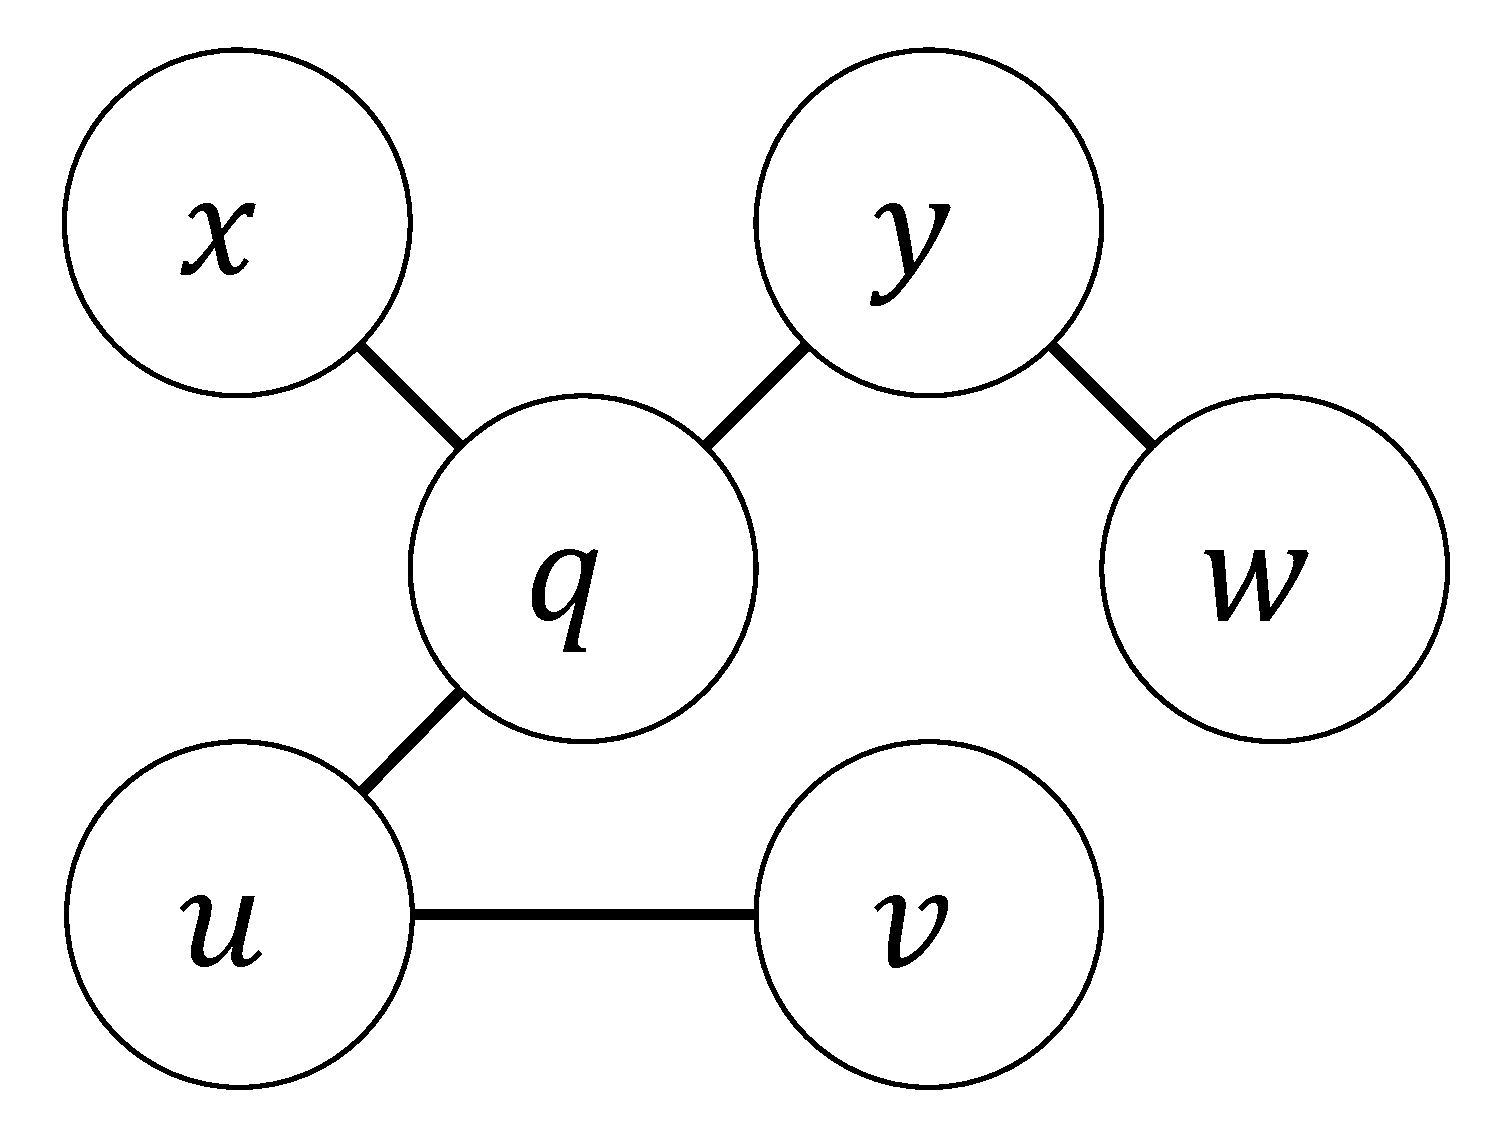
\includegraphics[width=0.3\textwidth]{figs/graph_example}
    \caption{An example of LinkedIn network}
    \label{fig:graph}
\end{figure}

Consider an example on LinkedIn to illustrate the skyline subspace queries on graph. In Figure~\ref{fig:graph}, a graph is represented by the LinkedIn connection network. Table~\ref{tab:skill_sets} shows the skills of each person of the LinkedIn network which can be treated as vertices with labels. 
Both of them together represent a \emph{label graph}. In Table~\ref{tab:skill_sets}, it shows that vertex $u$ has a skill of Accounting, vertex $w$ has skills of Bioinformatics and C++ and vertex $y$ has a skill of Bioinformatics. In this example, we want to compute the subspace skyline queries in $3$ hops.

\begin{table}[h]
    \centering
    \begin{tabular}{llll}
    \hline
        Distances & A & B & C \\ \hline
        $u$       & 0 & 2 & 3 \\ \hline
        $v$       & 1 & 3 & $\infty$ \\ \hline
        $w$       & 3 & 0 & 0 \\ \hline
        $x$       & 2 & 2 & 3 \\ \hline
        $y$       & 2 & 0 & 1 \\ \hline
        $z$       & 1 & 1 & 2 \\ \hline
    \end{tabular}
    \caption{\label{tab:distances_graph} distances between each person and each skill}
    
\end{table}

In the header row of Table~\ref{tab:distances_graph}, $A$, $B$ and $C$ stand for Accounting, Bioforinformatics and C++ respectively. The table shows the distances between each person and each skill. For example, the distance between $v$ and skill $B$ is $3$ because $y$ is the closest vertex to $v$ that contains label $B$ and the distance between $v$ and $y$ is $3$. Since C++ is not reachable by $v$ in $3$ hops, the distance between $v$ and $C$ is $\infty$. Each row of Table~\ref{tab:distances_graph} represents a \emph{label vector} of a vertex.
In this example, if the query point is $z$, the minimal skyline subspaces of $z$ are $(A, B)$ and $(A, C)$ because there is no such a vertex $w \in S$ that $w_{(A,B)}$ dominates $z_{(A,B)}$ or $w_{(A,C)}$ dominates $z_{(A,C)}$.


\section{Spatial Skyline Subspace Queries}

In this section, we will introduce spatial skyline subspace queries. Given a set of points in $2$-dimensional space. Some of the points will contain some labels. The distance between a point and a label is the Euclidean distance between that point and the closest point containing that label. Our goal is to compute the skyline subspace queries on this spatial setting.

\begin{definition}[Spatial Label Distance Vector]
Given a set of points $P$, the Label Distance Vector of a point $v$ is $LV_v=\left\{\left(l_i, dist_i\right)\right\}$, $i = 1 \ldots n$. $l_i$ is a reachable label from $v$. $dist_i$ is the Euclidean distance from vertex $v$ to the closest vertex that contains label $l_i$.
\end{definition}

\begin{definition}[Spatial Skyline Subspace Queries]
Given a set of points $P$ and a query point $q$, the skyline subspaces query on Euclidean space is to find all the \emph{minimal skyline subspaces} in terms of the spatial label distance vectors.
\end{definition}

\begin{table}[h]
    \centering
    \begin{tabular}{|l|l|}
    \hline
    Categories     & Spots \\ \hline
    Asian Food     & $u$     \\ \hline
    Breakfast      & $y, w$  \\ \hline
    Cafes          & $w$     \\ \hline
    \end{tabular}
    \caption{An example of spots with categories}
    \label{tab:spot_category} 
\end{table}


\begin{figure}[h]
    \centering
    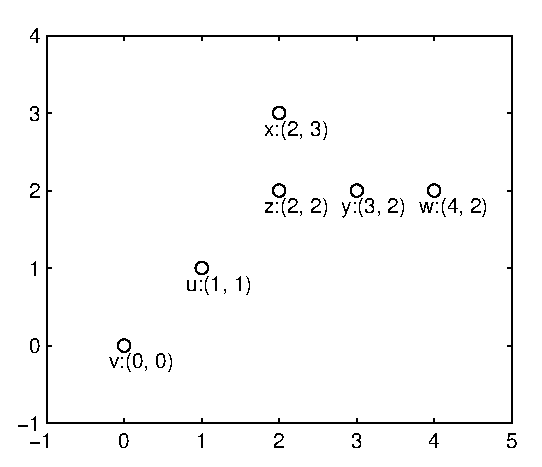
\includegraphics[width=0.5\textwidth]{figs/spatial_figure}
    \caption{An example of spatial locations of spots}
    \label{fig:spatial_map}
\end{figure}

Table~\ref{tab:spot_category} shows different spots with different categories. Figure~\ref{fig:spatial_map} shows the geometric locations of all spots. We consider each spot as a point in a $2$-dimensional space and the categories the spot contains as its labels.

\begin{table}[h]
    \centering
    \begin{tabular}{llll}
    \hline
    Distances & A & B & C \\ \hline
    $u$       & 0 & $\sqrt{5}$ & $\sqrt{10}$ \\ \hline
    $v$       & $\sqrt{2}$ & $\sqrt{13}$ & $\sqrt{18}$ \\ \hline
    $w$       & $\sqrt{10}$ & 0 & 0 \\ \hline
    $x$       & $\sqrt{5}$ & $\sqrt{2}$ & $\sqrt{5}$ \\ \hline
    $y$       & $\sqrt{5}$ & 0 & 1 \\ \hline
    $z$       & $\sqrt{2}$ & 1 & 2 \\ \hline
    \end{tabular}
    \caption{\label{tab:distances_spatial} Distances between each spot and each categories}
\end{table}

In the header row of Table~\ref{tab:distances_spatial}, $A$, $B$ and $C$ stand for Asian Food, Breakfast and Cafes respectively. The table shows the distances between each spot and each categories. In this example, if $z$ is the query point, then the minimal skyline subspaces are $(A, B)$ and $(A, C)$.



%% Copyright 1998 Pepe Kubon
%%
%% `two.tex' --- 2nd chapter for thes-full.tex, thes-short-tex from
%%               the `csthesis' bundle
%%
%% You are allowed to distribute this file together with all files
%% mentioned in READ.ME.
%%
%% You are not allowed to modify its contents.
%%

%%%%%%%%%%%%%%%%%%%%%%%%%%%%%%%%%%%%%%%%%%%%%%%%%
%
%     Chapter 4  
%
%%%%%%%%%%%%%%%%%%%%%%%%%%%%%%%%%%%%%%%%%%%%%%%%

\chapter{A Pruning-based Method On Graph}
\label{ch:graph}

In this chapter, we will introduce the algorithms to compute the skyline subspace queries. One way to solve this problem is to compute the label distance vectors of all the vertices first and enumerate all the subspaces to check whether the query vertex is a subspace skyline in those subspaces. This method could be very time consuming. In order to make the algorithm more efficient, we propose a bottom-up set enumeration algorithm and manage to avoid some unnecessary computations by applying some pruning techniques in our method.

\begin{table}[h]
\centering
\begin{tabular}{|l|p{11cm}|}
\hline
Symbol                      & Interpretation                                                                                                                                     \\ \hline
$q$                         & query vertex $q$                                                                                                                                   \\ \hline
$LV_v$                      & label distance vector of vertex $v$ representing the distances between $v$ and each label.                                                         \\ \hline
$\mathcal{B}$               & subspace $\mathcal{B}$                                                                                                                             \\ \hline
$\mathit{SDS}_u$            & strictly dominating subspace of $u$                                                                                                                \\ \hline
$\mathit{EQ}_u$             & equivalence subspace of $u$                                                                                                                        \\ \hline
$\mathit{CAND}_\mathcal{B}$ & dominating candidate set of subspace $\mathcal{B}$                                                                                                 \\ \hline
$(u, dom)$                  & element in dominating candidate set. $(u, dom) \in \mathit{CAND}_\mathcal{B}$ means that $u$ dominates query vertex $q$ in subspace $\mathcal{B}$. \\ \hline
$(u, eq)$                   & element in dominating candidate set. $(u, eq) \in \mathit{CAND}_\mathcal{B}$ means that $u$ dominates query vertex $q$ in subspace $\mathcal{B}$.  \\ \hline
\end{tabular}
    \caption{\label{font-table}Symbols Used in the Pruning-based Method on Graph}
    \label{tab:symbol_graph}
\end{table}

\section{BFS Label Collecting}
\label{sec:bfs-collect}
We collect the d-hop labels by Breadth-First-Search and get the \emph{label distance vector} of query vertex. The idea is that we start with our query vertex and traverse the graph in the Breadth First order. If we visit a vertex with a new label that we have not visited before, we update the corresponding entry of that label in \emph{label distance vector} to the distance from query vertex. The Breadth First Search process will end if all reachable vertices in $d$ hops has been visited. And we will get the \emph{label distance vector} of the query vertex when the BFS label collecting ends.

\begin{algorithm}[H]
  \caption{Label Collecting}\label{algo:blah}
  \begin{algorithmic}[1]
  \show\LOOP
    \REQUIRE A graph $G=(V,E)$, a list of label sets $F=\left\{L_v | v \in V\right\}$, the label sets of all vertices, a query vertex $q$, the number of hops $d$;
    \ENSURE The label distance vector $LV_q$ of the query vertex $q$;
    \STATE push $\left(q, 0\right)$ to $Q$
    \WHILE {$Q$ is not empty}
        \STATE $\left( v, dis\right)$ = de-queue $Q$
        \IF{$dis=d$}
            \STATE continue
        \ENDIF
        \FORALL {not visited neighbour $u$ of $v$}
            \STATE push $\left(u, dis+1\right)$ to $Q$
            \FORALL {label $l$ in $L_u$}
                \IF {($l$, $\ast$) not in $LV_q$}
                    \STATE add ($l$, $dis+1$) to $LV_q$
                \ENDIF
            \ENDFOR
        \ENDFOR
    \ENDWHILE
  \end{algorithmic}
\end{algorithm}

\section{Dominating Candidates Set}
\label{sec:bfs-collect}

By collecting the label in $d$ hops from the query vertex, we build the label distance vector of our query vertex. To avoid computing the label distance vectors of all other vertices to find the skyline subspaces, we define a concept of dominating candidates set to compute the skyline subspaces.

\begin{definition}[Dominating Candidates Set]
Given a subspace $\mathcal{B}$, the dominating candidates set of that subspace is the set of vertices that dominate the query vertex $q$ or equal to query vertex $q$ in subspace $\mathcal{B}$, denoted by $\mathit{CAND}_\mathcal{B}$.
\end{definition}

\begin{property}
\label{ppt:empty_cand}
If $\mathit{CAND}_\mathcal{B} = \emptyset$ or every vertex in $\mathit{CAND}_\mathcal{B}$ is equal to the query vertex $q$ in subspace $\mathcal{B}$, then $q$ is a skyline in subspace $\mathcal{B}$.
\end{property}

\begin{proof}
If $\mathit{CAND}_\mathcal{B} = \emptyset$ or every vertex in $\mathit{CAND}_\mathcal{B}$ is equal to the query vertex $q$ in subspace $\mathcal{B}$, then there is no vertex dominates the query vertex $q$ in $\mathit{CAND}_\mathcal{B}$.
$\mathit{CAND}_\mathcal{B}$ contains all the vertices that are not dominated by $q$. If all the vertices in $\mathit{CAND}_\mathcal{B}$ do not dominate $q$ in $\mathcal{B}$ then $q$ must be a skyline in subspace $\mathcal{B}$.
\end{proof}

Property~\ref{ppt:empty_cand}, shows that we can determine whether a subspace $\mathcal{B}$ is a \emph{skyline subspace} by checking the elements the \emph{dominating candidates set} of the subspace $\mathcal{B}$.


\subsection{Dominating Candidates Set of $1$-dimensional subspace}

We will introduce an algorithm to compute the \emph{dominating candidates set} of $1$-dimensional subspace. We will also introduce the concepts of \emph{Strictly Dominating Subspace} and \emph{Equivalence Subspace} which help us prune the unnecessary dominating candidates.

\begin{definition}[Strictly Dominate]
In a label graph, we say that label distance vector $LV_v=\left\{(l_i, dist_i)\right\}$ dominates label vector $LV_u=\left\{(l_i, dist_i^\prime)\right\}$, if and only if for all i, $dist_i < dist_i^\prime$.
\end{definition}

\begin{definition}[Strictly Dominating Subspace]
Strictly dominating subspace $\mathcal{B}$ is the maximal subspace such that given a vertex $u$, $u_\mathcal{B}$ strictly dominates query vertex $q_\mathcal{B}$ on subspace $\mathcal{B}$, denoted as $\mathit{SDS}_u$.
\end{definition}

\begin{definition}[Equivalence Subspace]
Equivalence subspace $\mathcal{B}$ is the maximal subspace such that given a vertex $u$, if $u_\mathcal{B}$ equals to the query vertex $q_\mathcal{B}$ in subspace $\mathcal{B}$, denoted as $\mathit{EQ}_u$.
\end{definition}

In this algorithm, we start from the vertices with labels and update the label distance vector of those vertices. In the next step, we push all the neighbours of those vertices into the queue and update their label distance vectors and keep going. 
\begin{algorithm}[h]
  \caption{Dominating Candidates Set On $1$-Dimensional Subspace}\label{algo:blah}
  \begin{algorithmic}[1]
  \show\LOOP
    \REQUIRE A graph $G=(V,E)$ and the label vector $LV_q$ of the query vertex $q$;
    \ENSURE Dominating Candidates Set $\mathit{CAND}$ in all one dimension subspace in $LV_q$, $\mathit{EQS}$ and $\mathit{SDS}$;
    \FORALL {vertex $v$ contains label $l$}
        \FORALL {$\left(l, dist\right)$ in $LV_q$}
            \STATE push $\left(v, 0\right)$ to $Q$
        \ENDFOR
    \ENDFOR
    \WHILE {$Q \not= \emptyset$}
        \FORALL {$\left(l, dist\right)$ in $LV_q$}
            \STATE $\left(v, dist_{v,l}\right)$ = de-queue $Q$
            
            \IF{$dist_{v,l} = dist$}
                \STATE add $\left(u, equal\right)$ to $\mathit{CAND}_l$
                \STATE add $l$ to $\mathit{EQS}_u$
                \STATE continue
            \ENDIF
            \STATE add $\left(u, dom\right)$ to $\mathit{CAND}_l$
            \STATE add $l$ to $\mathit{SDS}_u$
            \FORALL {not visited neighbour $u$ of $v$}
                \STATE push $\left(u, dist_{v,l}+1\right)$ to $Q$
            \ENDFOR
        \ENDFOR
    \ENDWHILE
  \end{algorithmic}
\end{algorithm}

\subsection{Running Example of Computing Dominating Candidates Set}

In this subsection, we will give an example of how the algorithm of finding \emph{dominating candidates set on $1$-dimensional subspace} works. We will also show how the \emph{strictly dominating subspace} and the \emph{equivalence subspace} of each vertex is built.

\begin{figure}[H]
    \centering
    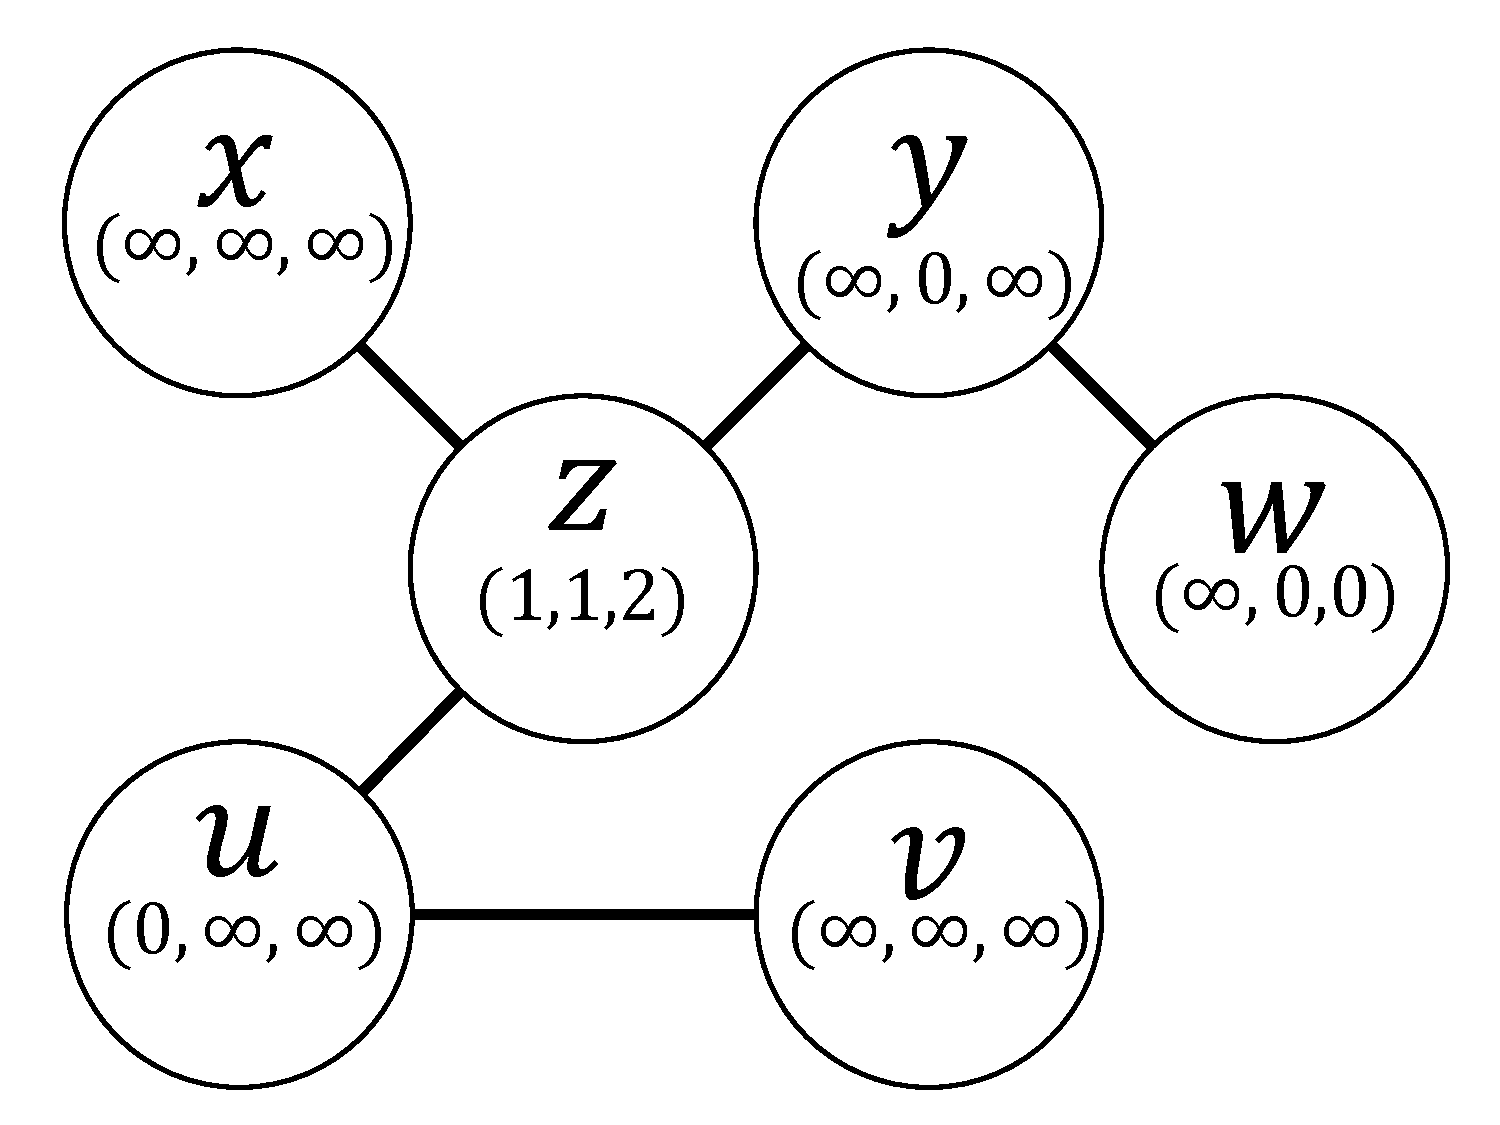
\includegraphics[width=0.5\textwidth]{figs/graph_example_1}
    \caption{\label{font-figure}label distance vector on the first iteration}
    \label{fig:cand_step1}
\end{figure}

\begin{table}[H]
    \centering
    \begin{tabular}{|l|l|l|}
    \hline
      & SDS         & EQS         \\ \hline
    u & A           & $\emptyset$ \\ \hline
    v & $\emptyset$ & $\emptyset$ \\ \hline
    w & BC          & $\emptyset$ \\ \hline
    x & $\emptyset$ & $\emptyset$ \\ \hline
    y & B           & $\emptyset$ \\ \hline
    \end{tabular}
    \caption{\label{font-table}SDS and EQS of each vertex on the first iteration}
    \label{tab:sds_step1}
\end{table}

\begin{table}[H]
    \centering

    \begin{tabular}{|l|l|}
    \hline
    Subspaces & Dominating Candidates \\ \hline
    A         & $(u, dom)$            \\ \hline
    B         & $(w, dom), (y, dom)$            \\ \hline
    C         & $(w, dom)$            \\ \hline
    \end{tabular}
    \caption{\label{font-table}dominating candidates set of each $1$-dimensional subspace on the first iteration}
    \label{tab:cand_set_step1}
\end{table}

Consider the LinkedIn network represented by Table~\ref{tab:skill_sets} and Figure~\ref{fig:graph} as our running example. Again, we take $z$ as the query vertex. The label distance vectors of all vertices are originally initialized as $\infty$. As shown in Figure~\ref{fig:cand_step1}, we start from the vertices with labels and mark the corresponding entries of the label distance vectors of those vertices as $0$. 
We add the label $A$ to $\mathit{SDS}_u$ because $u$ dominates the query vertex $z$ in dimension $A$. Table~\ref{tab:sds_step1} shows the $\mathit{SDS}$ and $\mathit{EQS}$ of all the vertices on the first iteration.
In the first iteration, since $u$ dominates $z$ in the $1$-dimensional subspace $A$, we add $(u, dom)$ to the dominating candidate set $\mathit{CAND}_A$ as shown in Table~\ref{tab:cand_set_step1}.

\begin{figure}[H]
    \centering
    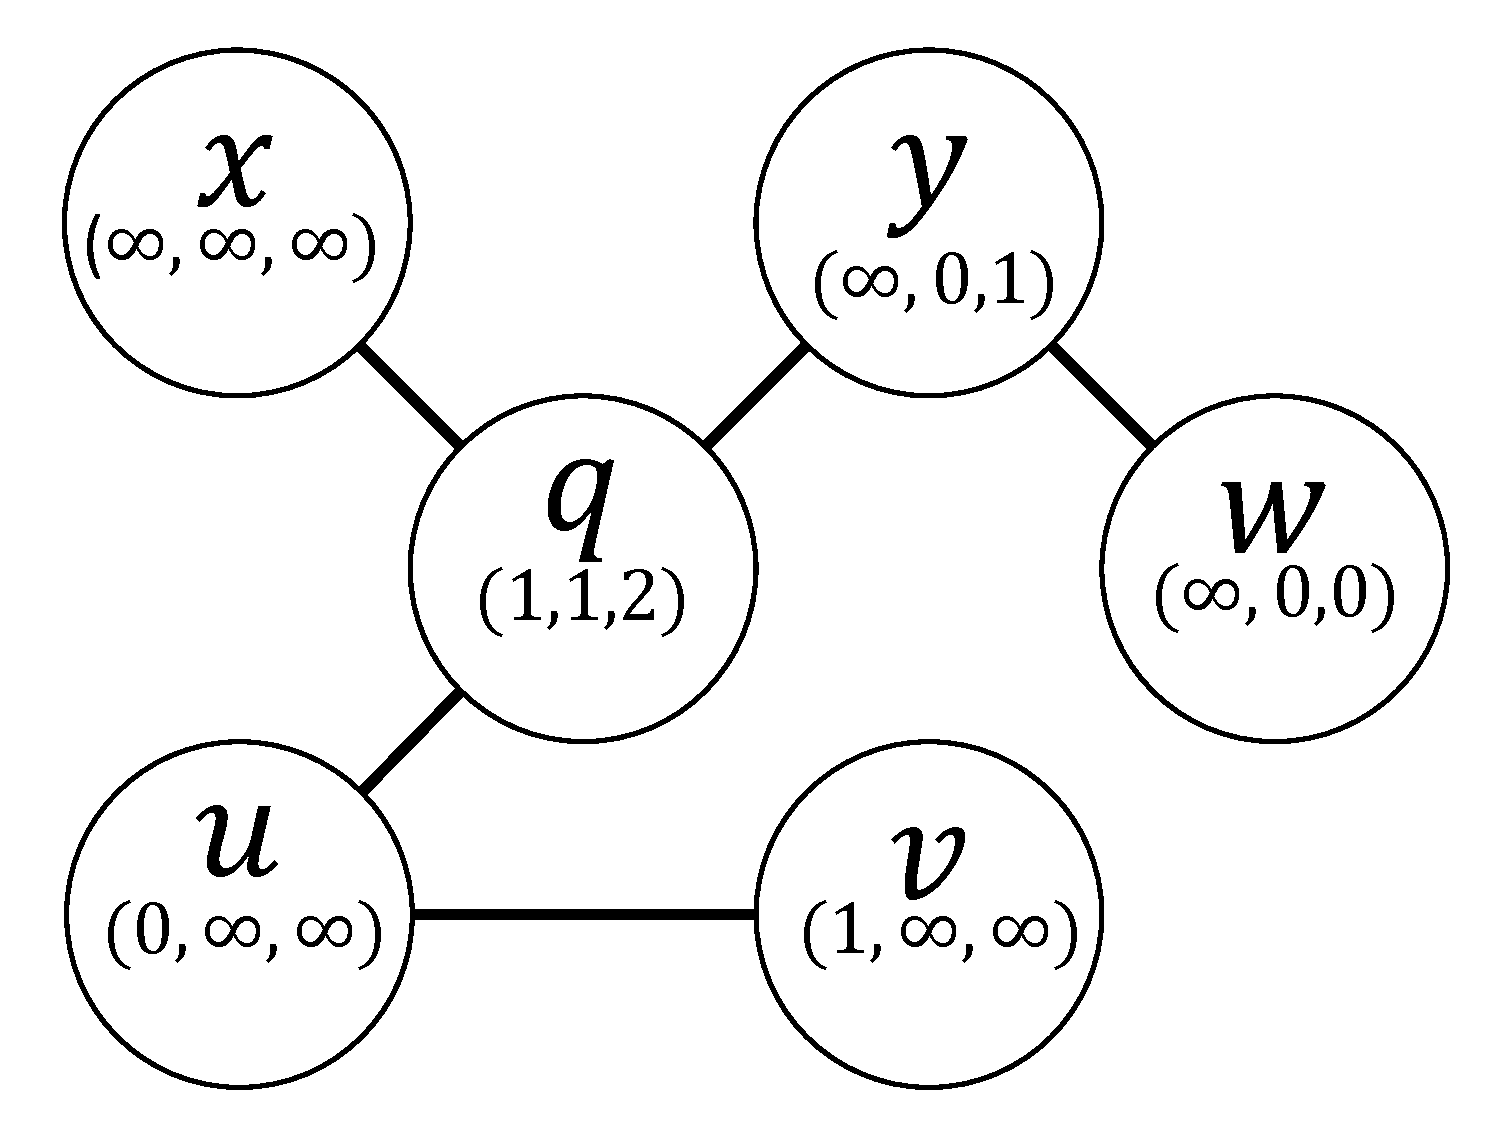
\includegraphics[width=0.5\textwidth]{figs/graph_example_2}
    \caption{\label{font-figure}label distance vector on second iteration}
    \label{fig:cand_step2}
\end{figure}

\begin{table}[H]
    \centering
    \begin{tabular}{|l|l|l|}
    \hline
      & SDS         & EQS         \\ \hline
    u & A           & $\emptyset$ \\ \hline
    v & $\emptyset$ & A           \\ \hline
    w & BC          & $\emptyset$ \\ \hline
    x & $\emptyset$ & $\emptyset$ \\ \hline
    y & BC          & $\emptyset$ \\ \hline
    \end{tabular}
    \caption{\label{font-table}SDS and EQS of each vertex on the second iteration}
    \label{tab:sds_step2}
\end{table}

\begin{table}[H]
    \centering

    \begin{tabular}{|l|l|}
    \hline
    Subspaces & Dominating Candidates \\ \hline
    A         & $(u, dom), (v, eq)$            \\ \hline
    B         & $(w, dom), (y, dom)$            \\ \hline
    C         & $(w, dom), (y, dom)$            \\ \hline
    \end{tabular}
    \caption{\label{font-table}dominating candidates set of each $1$-dimensional subspace on the second iteration}
    \label{tab:cand_set_step2}
\end{table}


Then, we explore the graph in breadth first order. On the second iteration, as shown in Figure~\ref{fig:cand_step2}, we visit the neighbours of the vertices that have been visited on the first iteration and update the corresponding entries of their label distance vectors. Table~\ref{tab:sds_step2} shows that subspace $A$ has been added to $\mathit{EQS}_v$ because on the second iteration we update the distance between $v$ and label $A$ to $2$ which is equal to distance between $z$ and label $A$. For the same reason, we add $(v, eq)$ to $\mathit{CAND}_A$ as shown in Table~\ref{tab:cand_set_step2}. It means that in $1$-dimensional subspace $A$, $v$ is equal to $z$ and it is still possible for $v$ to dominates $z$.

After $2$ iterations, the process of building the  dominating candidate sets of all $1$-dimensional subspace ends. We also finish building the \emph{strictly dominating subspace} and \emph{equivalence subspace} of all the vertices on graph. In figure~\ref{tab:d_hops_distance}, we collect the $3$-hop labels by Breadth-First-Search and get the label vector. By this point, if the value of label $l$ in label distance vertex of vertex $v$ is $\infty$, then it means the distance between label $l$ and vertex $v$ is longer than the distance between the label $l$ and the query vertex $q$.

\begin{table}[h]
    \centering
    \begin{tabular}{llll}
    \hline
    Distances & A & B & C \\ \hline
    $u$       & 0 & $\infty$ & $\infty$ \\ \hline
    $v$       & 1 & $\infty$ & $\infty$ \\ \hline
    $w$       & $\infty$ & 0 & 0 \\ \hline
    $x$       & $\infty$ & $\infty$ & $\infty$ \\ \hline
    $y$       & $\infty$ & 0 & 1 \\ \hline
    $z$       & 1 & 1 & 2 \\ \hline
    \end{tabular}
    \caption{\label{font-table} distances between each person and each skill in 2-hop}
    \label{tab:d_hops_distance}
\end{table}

Although some information is still missing (equal to $\infty$), we are still able to get the mininmal skyline subspaces of $z$: $(A, B)$ and $(A, C)$ from the Table~\ref{tab:d_hops_distance}.

\section{Dominating Candidates Pruning}

In this section, we will introduce a way to prune the unnecessary vertices using the \emph{strictly dominating subspace} $SDS$ and the \emph{equivalence subspace} of the vertices.

\begin{property}
\label{ppt:prune_cand}
Pruning a vertex $u$ from $\mathit{CAND}$ that $\exists v, (SDS_u \cup EQS_u \subseteq SDS_v \cup EQS_v) \wedge (SDS_u \subseteq SDS_v)$, does not affect the result. Therefore, $u$ can be pruned by $v$.
\end{property}

\begin{proof}
Let $u$ be a vertex that $\exists v, (SDS_u \cup EQS_u \subseteq SDS_v \cup EQS_v) \wedge (SDS_u \subseteq SDS_v)$. For the query vertex $q$ in any subspace $\mathcal{B}$, there are three different cases.\\
Case 1: $q$ is a skyline in subspace $\mathcal{B}$. Then $\mathit{CAND}_\mathcal{B}$ does not contain any elements. Pruning $u$ from $\mathit{CAND}$ does not change the result.\\
Case 2: $q$ is not a skyline in subspace $\mathcal{B}$ and $q$ is dominated by a vertex $w$, removing $u$ does not change the result.\\
Case 3: $q$ is not a skyline in subspace $\mathcal{B}$ and $q$ is dominated by vertex $u$, then $(\mathcal{B} \subseteq EQS_u \cup SDS_u) \wedge (\mathcal{B} \cap SDS_u \not= \emptyset)$, and there exists such a $v$ that ($SDS_u \cup EQS_u \subseteq SDS_v \cup EQS_v) \wedge (SDS_u \subseteq SDS_v)$. And $(\mathcal{B} \subseteq EQS_v \cup SDS_v) \wedge (\mathcal{B} \cap SDS_v \not= \emptyset)$ is satisfied.\\
Therefore $v$ also dominates $q$ and removing $u$ from $CAND$ does not affect the result.
\end{proof}

One observation is that the unnecessary points is very likely to be pruned by the neighbours of the query vertex $q$. The intuition is that the neighbours of query vertex $q$ will have larger \emph{Strictly Dominating Set} because the query vertex $q$ collects the labels directly from its neighbours and the neighbours strictly dominate the query vertex in subspaces of those labels.
By the Property~\ref{ppt:prune_cand} and the observation above we develop a $1$-hop pruning algorithm. In Algorithm~\ref{algo:pruning_graph}, we compare the $\mathit{SDS}$ and $\mathit{EQS}$ values of neighbours of the query vertex $q$ to all the vertex in the graph in order to prune the some of the candidates in the \emph{dominating candidate sets}.

\begin{algorithm}[H]
  \caption{1-hop Pruning}
  \label{algo:pruning_graph}
  \begin{algorithmic}[1]
  \show\LOOP
    \REQUIRE Strictly Dominating Subspace $\mathit{SDS}$, Equivalence Subspace $\mathit{EQS}$, Dominating Candidates $\mathit{CAND}$, query vertex $q$, graph $G=(V, E)$;
    \ENSURE Pruned Dominating Candidates $\mathit{CAND}$;
    \STATE s = $\left\{v|e(v, q) \in E \wedge (\forall u, e(u, q) \in E \wedge SDS_v \not\subset SDS_u)\right\}$
    
    \FORALL {$(l, dist)$ in $LV_q$}
        \FORALL {$u$ in $\mathit{CAND}_l$}
            \FORALL {$v$ in $s$}
                \IF {$u \not= v \wedge SDS_u \cup EQS_u \subseteq SDS_v \cup EQS_v \wedge SDS_u \subseteq SDS_v$}
                    \STATE delete $u$ from $\mathit{CAND}_l$
                \ENDIF
                
            \ENDFOR
        \ENDFOR
    \ENDFOR
  \end{algorithmic}
\end{algorithm}

\begin{table}[h]
    \centering
    \begin{tabular}{|l|l|l|l|}
    \hline
    Dim & $SDS$       & $EQS$       & $SDS \cup EQS$ \\ \hline
    $u$ & A           & $\emptyset$ & A              \\ \hline
    $v$ & $\emptyset$ & A           & A              \\ \hline
    $w$ & BC          & $\emptyset$ & BC             \\ \hline
    $x$ & $\emptyset$ & $\emptyset$ & $\emptyset$    \\ \hline
    $y$ & BC          & $\emptyset$ & BC             \\ \hline
    \end{tabular}
    \caption{\label{font-table} the $SDS$ and $EQS$ of each vertex}
    \label{tab:SDS_EQS}
\end{table}

Table~\ref{tab:SDS_EQS} shows the $SDS$ and $EQS$ of all vertices on the graph. We can prune the unnecessary vertices from the \emph{dominating candidate set} according this table. By Property~\ref{ppt:prune_cand}, vertex $v$ can be pruned by $v$ and vertex $w$ and $y$ can be pruned by each other.

\begin{table}[h]
    \centering
    \begin{tabular}{lllll}
    \hline
    Distances & A & B & C & Pruned By\\ \hline
    $u$       & 0 & $\infty$ & $\infty$ &\\ \hline
    $v$       & 1 & $\infty$ & $\infty$ & $u$\\ \hline
    $w$       & $\infty$ & 0 & 0 & $y$\\ \hline
    $x$       & $\infty$ & $\infty$ & $\infty$ & $u$\\ \hline
    $y$       & $\infty$ & 0 & 1 & \\ \hline
    $z$       & 1 & 1 & 2 &\\ \hline
    \end{tabular}
    \caption{\label{font-table} label distance vector after 1-hop pruning}
    \label{tab:lv_pruned}
\end{table}

\begin{table}[h]
    \centering
    \begin{tabular}{|l|l|}
    \hline
    Subspaces & Dominating Candidates \\ \hline
    A         & $(u, dom)$            \\ \hline
    B         & $(y, dom)$            \\ \hline
    C         & $(y, dom)$            \\ \hline
    \end{tabular}
    \caption{\label{font-table} Pruned dominating candidate set of $1$-dimensional subspace}
    \label{tab:dom_cand_pruned}
\end{table}

By Table~\ref{tab:lv_pruned}, $v$ and $x$ can be pruned by $u$. Also, $y$ can be pruned by $w$. Table~\ref{tab:lv_pruned} show the vertices to be pruned and their label distance vectors. Although $w$ seems to be a better vertex (because $w$ dominates $y$),  the vertex $w$ is pruned by the vertex $y$ because both vertex $y$ and vertex $w$ have the same \emph{strictly dominating subspace} and \emph{equivalence subspace} and $y$ is a $1$-hop neighbour of the query vertex $q$. Table~\ref{tab:dom_cand_pruned} shows the dominating candidates set of $1$-dimensional subspace after the $1$-hop neighbour pruning.

\subsection{Dominating Candidate Set on Multi-dimensional Subspace}

We generate the dominating candidate set on multi-dimensional subspace by intersecting the smaller dominating candidate sets. Since each element in the CAND set of subspace $\mathcal{B}$ has a property \emph{dom} or \emph{eq} representing if that element is dominating query vertex $q$ in subspace $\mathcal{B}$ or equal to the query vertex $q$ in subspace $\mathcal{B}$, we define the CAND set intersection in the following way.

\begin{definition}[CAND Set Intersection]
\label{def:cand_intersect}
\begin{equation}
\begin{split}
\mathit{CAND}_{\mathcal{A} \cup \mathcal{B}} &= \mathit{CAND}_\mathcal{A} \cap \mathit{CAND}_\mathcal{B}\\
           &= \left\{(u, OR(x, y)) |\forall u, (u, x)\in \mathit{CAND}_\mathcal{A} \wedge (u, y)\in \mathit{CAND}_\mathcal{B} \right\}
\end{split}
\end{equation}
where $OR(x, y) = equal$ if $x = equal$ and $y = equal$, otherwise, $OR(x, y) = dom$.
\end{definition}

For example, consider two dominating candidate sets $\mathit{CAND}_\mathcal{A} = \left\{(u, dom)\right\}$ and $\mathit{CAND}_\mathcal{B} = \left\{(u, eq)\right\}$. And we want to compute the CAND intersection of these two dominating candidates sets $\mathit{CAND}_\mathcal{A} \cap \mathit{CAND}_\mathcal{B}$. 
Both $\mathit{CAND}_\mathcal{A}$ and $\mathit{CAND}_\mathcal{B}$ contain the element $u$. 

In the other words, vertex $u$ dominates query vertex $z$ in subspace $\mathcal{A}$ and vertex $u$ is equal to query vertex $q$ in subspace $\mathcal{B}$. 
Therefore, vertex $u$ dominates query vertex $q$ in the subspace $\mathcal{A} \cup \mathcal{B}$ because $u$ is less than $q$ in at least one dimension of $\mathcal{A} \cup \mathcal{B}$ ($u$ dominates $q$ in $\mathcal{A}$). By the Definition~\ref{def:cand_intersect}, we can also get the same answer $\mathit{CAND}_{\mathcal{A} \cup \mathcal{B}}$ = $\mathit{CAND}_\mathcal{A} \cap \mathit{CAND}_\mathcal{B} = \left\{(u, dom)\right\}$.


\subsection{Buttom-up Subspace Eumeration}

In this section, we will introduce a buttom-up algorithm to compute the dominating candidate set from low dimensional subspace to high dimensional subspace.
This algorithm is inspired by the Apriori algorithm for mining Association rules~\cite{agrawal1996fast}. A similar buttom-up algorithm has also been used in enumerating different subspaces in subspace clustering~\cite{agrawal1998automatic}.

\begin{property}
If in a k-dimensional subspace $\mathcal{B}$, $\mathit{CAND}_\mathcal{B}$ contain a set of vertices $S$, then in any (k-1)-dimensional projection $\mathcal{C}$ of $B$, $\mathit{CAND}_\mathcal{C}$ also contains the set of vertices $S$.
\end{property}

\begin{proof}
If a vertex $v$ in $\mathit{CAND}_\mathcal{B}$, where space $\mathcal{B}$ is a k-dimensional subspace, then the vertex $v$ is not greater than query vertex $q$ in any dimension of space $\mathcal{B}$. For any (k-1)-dimensional projection $\mathcal{C}$ of $B$, the vertex $v$ is also is not greater than query vertex $q$ in any dimension of projection $\mathcal{C}$. Therefore, in projection $\mathcal{C}$, $\mathit{CAND}_\mathcal{C}$ contains the vertex $v$.
\end{proof}

The algorithm compute the dominating candidates set level by level. We already introduce an algorithm to compute the all the dominating candidates set on all $1$-dimensional subspaces. Having all the dominating candidates sets on all $(k-1)$-dimensional subspaces, we are able to construct the possible dominating candidates sets on $k$-dimensional subspaces $C_k = \left\{\mathcal{A} \cup \left\{b\right\} | \mathcal{A} \in L_{k-1} \wedge b \in \bigcup L_{k-1} \wedge b \notin \mathcal{A} \right\}$.

\begin{algorithm}[H]
  \caption{Subspace Eumeration}\label{algo:blah}
    \begin{algorithmic}[1]
  \show\LOOP
    \REQUIRE Dominating Candidates $\mathit{CAND}$ of all one dimension subspaces in $LV_q$;
    \ENSURE A set of subspaces $SUB$ where query vertex $q$ is a skyline;
        \FORALL {$\left(l, dist\right)$ in $LV_q$}
            \STATE if $\exists u, (u, dom)\in \mathit{CAND}_l$, add $l$ to $SUB$, else add $l$ to $L_1$
        \ENDFOR
        \STATE $k$ = 2
        
        \WHILE {$L_{k-1} \not= \emptyset$}
        
            \STATE $C_k = \left\{\mathcal{A} \cup \left\{b\right\} | \mathcal{A} \in L_{k-1} \wedge b \in \bigcup L_{k-1} \wedge b \notin \mathcal{A} \right\}$
            
            \FORALL{$\mathcal{C}$ in $C_k$}
                \FORALL{(k-1)-projection $\mathcal{S}$ of $\mathcal{C}$ do}
                    \IF {$\mathcal{S} \notin L_{k-1}$}
                        \STATE delete $\mathcal{C}$ from $C_k$
                        
                    \ENDIF
                \ENDFOR
            \ENDFOR
            
            \FORALL{$\mathcal{C}$ in $C_k$}
                \STATE Let $b$ be the last element in $c$
                \STATE $CAND_\mathcal{C}$ = $CAND_b \cap CAND_{\mathcal{C}-\left\{b\right\}}$
                \STATE if $CAND_l$ is empty, add $l$ to $SUB$, else add $l$ to SUB
            \ENDFOR
            
            \STATE $k$ = $k$ + 1
        \ENDWHILE
        \RETURN SUB
  \end{algorithmic}
\end{algorithm}

We still consider the LinkedIn network represented by Table~\ref{tab:skill_sets} and Figure~\ref{fig:graph} as our running example. By running the \emph{set enumeration} algorithm we get the dominating candidate set in all subspaces in Table~\ref{tab:sub_dom_cand_pruned}.

\begin{table}[H]
    \centering
    \begin{tabular}{|l|l|l|}
    \hline
    Subspaces & Dominating Candidates & Generated By \\ \hline
    A         & $(u, dom)$  &              \\ \hline
    B         & $(w, dom)$  &              \\ \hline
    C         & $(w, dom)$  &              \\ \hline
    AB        & $\emptyset$           & $A \cap B$   \\ \hline
    AC        & $\emptyset$           & $A \cap C$   \\ \hline
    BC        & $(w, dom)$            & $B \cap C$   \\ \hline
    \end{tabular}
    \caption{\label{font-table} dominating candidates in all subspaces}
    \label{tab:sub_dom_cand_pruned}
\end{table}

As shown in Table~\ref{tab:sub_dom_cand_pruned}, $\mathit{CAND}_{BC}$ is computed by $\mathit{CAND}_{B} \cap \mathit{CAND}_{C}$, $\mathit{CAND}_{AB}$ is computed by $\mathit{CAND}_{A} \cap \mathit{CAND}_{B}$ and $\mathit{CAND}_{AC}$ is computed by $\mathit{CAND}_{A} \cap \mathit{CAND}_{C}$. In this example, $\mathit{CAND}_{BC} = \mathit{CAND}_B \cap \mathit{CAND}_C = \left\{(w, dom)\right\}$, $\mathit{CAND}_{AB} = \emptyset$ and $\mathit{CAND}_{AC} = \emptyset$.
The query vertex $z$ is a skyline on subspaces $AB$ and $BC$ because their dominating candidates sets are all empty.

%% Copyright 1998 Pepe Kubon
%%
%% `two.tex' --- 2nd chapter for thes-full.tex, thes-short-tex from
%%               the `csthesis' bundle
%%
%% You are allowed to distribute this file together with all files
%% mentioned in READ.ME.
%%
%% You are not allowed to modify its contents.
%%

%%%%%%%%%%%%%%%%%%%%%%%%%%%%%%%%%%%%%%%%%%%%%%%%%
%
%     Chapter 5   
%
%%%%%%%%%%%%%%%%%%%%%%%%%%%%%%%%%%%%%%%%%%%%%%%%

\chapter{Spatial Skyline Subspace}
\label{ch:spatial_skyline_subspace}

In this chapter, we will introduce the algorithms to compute the spatial skyline subspace queries. In the computation of spatial skyline subspace skyline queries, we use the same set enumeration framework as shown in Chapter~\ref{ch:graph}. However, in this chapter we introduce a different method to prune the unnecessary \emph{dominating candidates} based on some geometric property of skyline subspace.

\section{Label Collecting in Radius $D$}
We assume that the data points are indexed in R-tree. In R-tree we can get all points in a certain rectangle efficiently. By indexing the data points in R-tree, if we want access the neighbouring points of certain query point $q$, we can query the square with center $q$ in R-tree without accessing the whole set of data points. We compute query point $q$'s label distance vector $LV_q$ by checking the labels of the points in rectangle with upper-left corner point $(p.x - D, p.y - D)$ and lower-right corner point $(p.x + D, p.y + D)$. Then we collect the labels within distance $D$ as the label distance vector $LV_q$.

\section{Dominating Candidates in Spatial Subspace Skyline}

In this section, we will show an algorithm to compute the $\mathit{CAND}$ of all $1$-dimensional subspaces. We enumerate every point $v$ in the data set and build the label distance vector $LV_v$ of the point $v$ by querying square centering in point $v$.

\begin{algorithm}[H]
  \caption{Dominating Candidates}\label{algo:blah}
  \begin{algorithmic}[1]
  \show\LOOP
    \REQUIRE R-tree $R$ that indexes the spatial points and label distance vector $LV_q$ of query point $q$;
    \ENSURE Dominating Candidates Set $\mathit{CAND}$ of all $1$-dimensional subspaces, $\mathit{SDS}$ and $\mathit{EQS}$ of all points;
    \FORALL {$\left(l, dist\right)$ in $LV_q$}
        \FORALL {point $p$ contains label $l$}
            \STATE $rec = R.query(p.x-dist, p.y-dist, p.x+dist, p.y+dist)$
            \FORALL {point $u$ in $rec$}
                \STATE $d$ = $distance(v, p)$
                \IF {$d < dist$}
                    \STATE add$(u, dom)$ to $\mathit{CAND}_l$
                    \STATE add$l$ to $\mathit{SDS}_u$
                \ENDIF
                \IF {$d == dist$}
                    \STATE add$(u, eq)$ to $\mathit{CAND}_l$
                    \STATE add$l$ to $\mathit{EQS}_u$
                \ENDIF
            \ENDFOR
            
        \ENDFOR
    \ENDFOR
  \end{algorithmic}
\end{algorithm}

\section{Same Region Pruning}
After getting the list of dominating candidate sets and the $\mathit{SDS}$ and $\mathit{EQS}$ of all points, we can prune some unnecessary candidate points of the dominating candidate sets. By Property~\ref{ppt:prune_cand}, we can see that if two points $u$ and $v$ have the same $\mathit{SDS}_u$ and $\mathit{SDS}_v$ and they have the same $\mathit{EQS}_u$ and $\mathit{EQS}_v$, then one of the point $u$ and $v$ can be pruned by the other.

We will show an example of how the spatial points can be pruned from the dominating candidate set. In Figure~\ref{fig:circle_example}, point $q$ represents the query point, point $A$ represents a point with label $A$ and point $B$ represents a point with label $B$. $r_{A}$ is the distance between query point $q$ and label $A$ and $r_{B}$ is the distance between query point $q$ and label $B$. The blue points ($v_1$ and $v_2$) dominate the query point $q$ in the $1$-dimensional subspace $A$. The green points ($v_5$ and $v_6$) dominate the query point $q$ in subspace $B$. The red points ($v_3$ and $v_4$) dominate the query point $q$ in subspace $(A, B)$. In this example, the points with the same colors ($v_1$ and $v_2$, $v_3$ and $v_4$, $v_5$ and $v_6$) have the same \emph{strictly dominating subspace} $\mathit{SDS}$ and the same \emph{equivalence subspace} $\mathit{EQS}$. Therefore, we can keep one of them of each color as a representative and prune the others from the \emph{dominating candidate set}.


\begin{figure}[h]
    \centering
      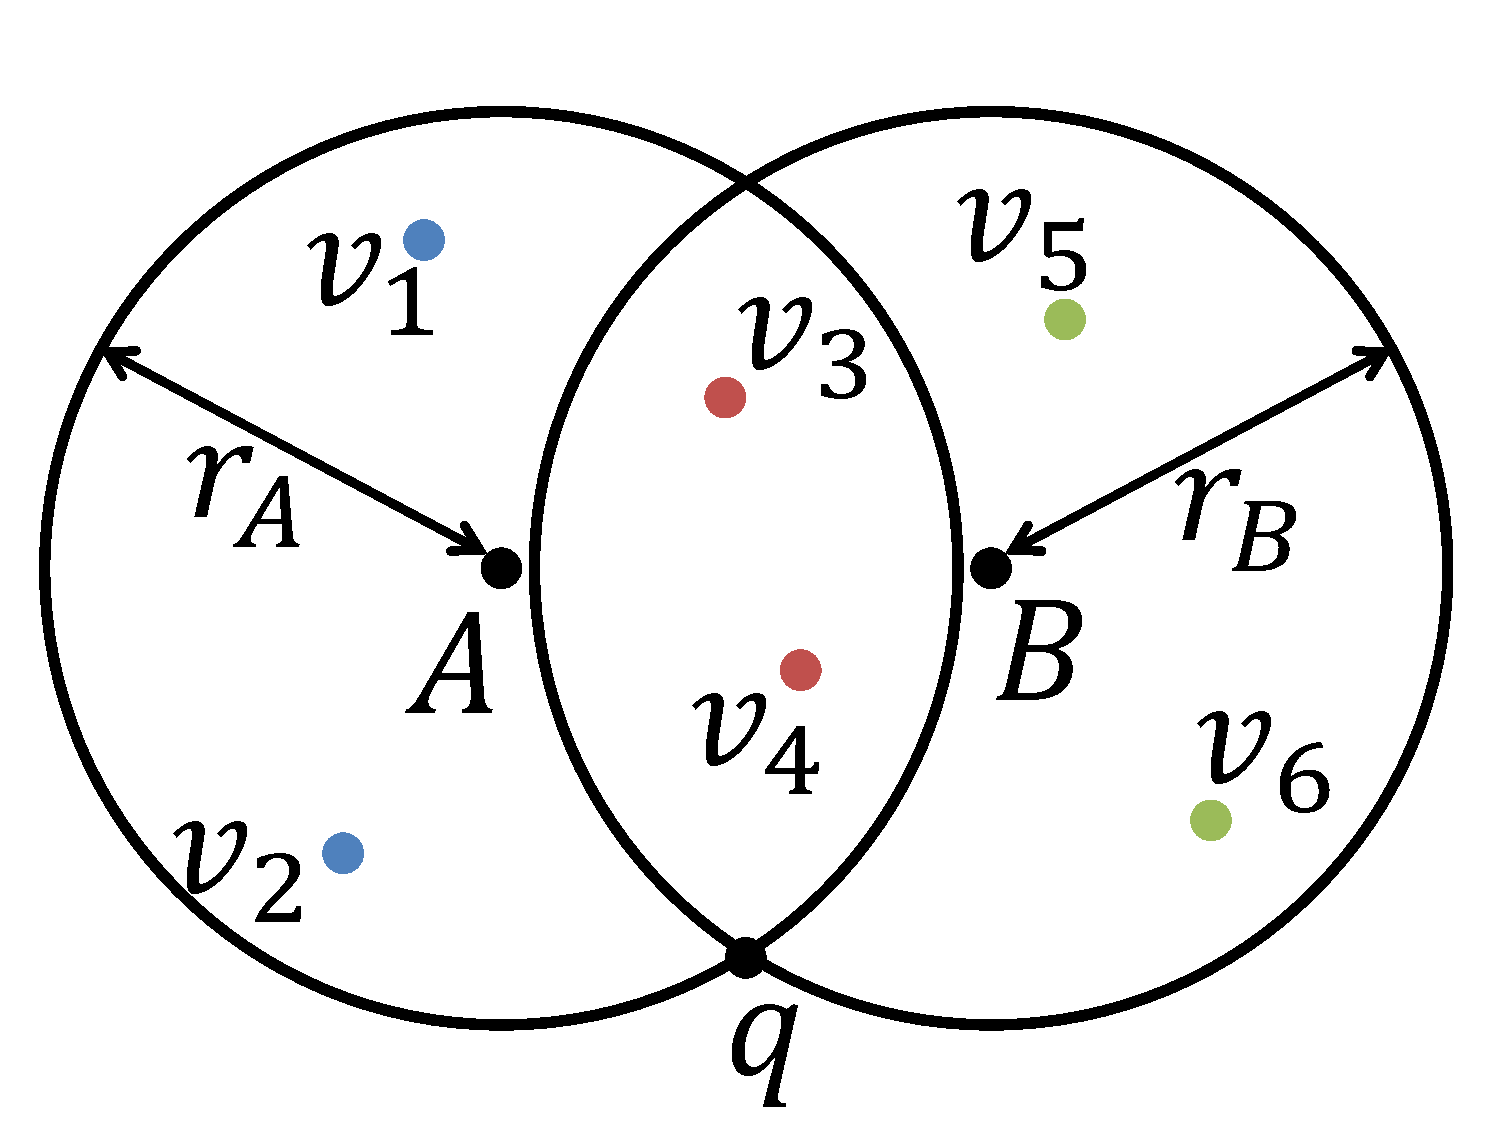
\includegraphics[width=0.5\textwidth]{figs/Circle_Spatial_Example}
    \caption{We can pick one candidate for each region (with same color) and eliminate the others.}
    \label{fig:circle_example}
\end{figure}


\begin{algorithm}[H]
  \caption{Same Region Pruning}\label{algo:blah}
  \begin{algorithmic}[1]
  \show\LOOP
    \REQUIRE Dominating Candidates $CAND$, query vertex $q$, graph $G=(V, E)$;
    \ENSURE Pruned Dominating Candidates $CAND$;
    \FORALL {$(l, dist)$ in $LV_q$}
        \FORALL {$u$ in $CAND_l$}
            \IF {$u$ is in the same region as other points}
                \STATE delete $u$ from $CAND_l$
            \ENDIF
        \ENDFOR
    \ENDFOR
  \end{algorithmic}
\end{algorithm}
And we will use the same set-enumeration method to compute dominating candidates to get the skyline subspace.




%% Copyright 1998 Pepe Kubon
%%
%% `two.tex' --- 2nd chapter for thes-full.tex, thes-short-tex from
%%               the `csthesis' bundle
%%
%% You are allowed to distribute this file together with all files
%% mentioned in READ.ME.
%%
%% You are not allowed to modify its contents.
%%

%%%%%%%%%%%%%%%%%%%%%%%%%%%%%%%%%%%%%%%%%%%%%%%%%
%
%     Chapter 6  
%
%%%%%%%%%%%%%%%%%%%%%%%%%%%%%%%%%%%%%%%%%%%%%%%%

\chapter{Experiments}
\label{ch:exp}

To validate the effectiveness and efficiency of our two methods named GP and MHI, we first report the experimental results with respect to Jaccard similarity on synthetic data sets in Section~\ref{sec:syn-data}. The results on two real data sets on market basket data and click stream data are presented in Section~\ref{sec:real-data}. We also show the performance of the pruning algorithms on Cosine similarity and edit distance in Section~\ref{sec:other-measure} using the click stream data set. All methods are implemented in Python and all experiments are conducted on a PC computer with Intel Core 2 Duo E8400 3.00GHz CPU and 8GB main memory running 64-bit Microsoft Windows 7.


%%%%%% Synthetic Data Set %%%%%%
\section{Results on Synthetic Data Sets}
\label{sec:syn-data}
The following results are generated using the IBM Quest data generator\footnote{\url{http://www.cs.loyola.edu/~cgiannel/assoc_gen.html}}. We conduct experiments to test the efficiency and accuracy of our methods regarding the following parameters. 
% We use the following notations for ease of presentation: 

\begin{itemize}
\item $k$ - top-$k$; 
\item $n$ - number of items per query/ average number of items per object.
\item $|\Sigma|$ - lexicon size;
\item $m$ - number of objects;
\item $l$ - number of different hash functions/ random permutations.
\end{itemize}

%%% test on IBM Quest data %%%

\begin{figure*}[htb]
\centering
\subfigure{% a
\label{legend}

\includegraphics[width=1\textwidth]{fig/legend_efficiency.eps}}
\quad
\setcounter{subfigure}{0}
\subfigure[Large $|\Sigma|$]{% a
\label{questLLVka}
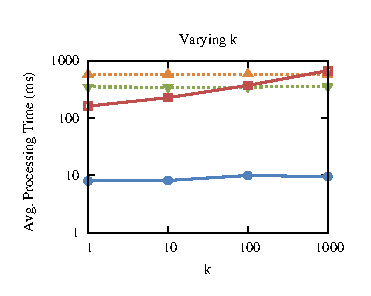
\includegraphics[width=0.45\textwidth]{fig/vary_k_large.eps}}
\quad
\subfigure[Small $|\Sigma|$]{% b
\label{questSLVka}
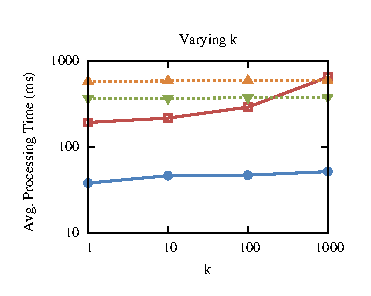
\includegraphics[width=0.45 \textwidth]{fig/vary_k_small.eps}}
\quad
\subfigure[]{% c
\label{questVsigmaa}
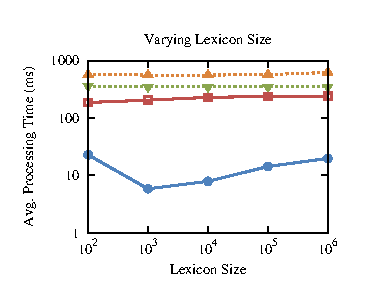
\includegraphics[width=0.45 \textwidth]{fig/vary_lexicon.eps}}
\quad
\subfigure[]{% g
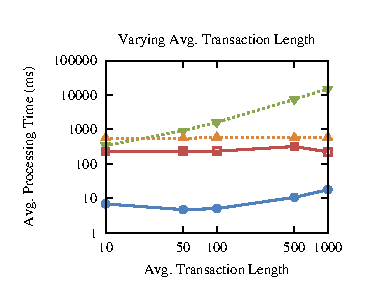
\includegraphics[width=0.45 \textwidth]{fig/vary_txn_len.eps} 
\label{questVna}}
\quad
\subfigure[]{% h
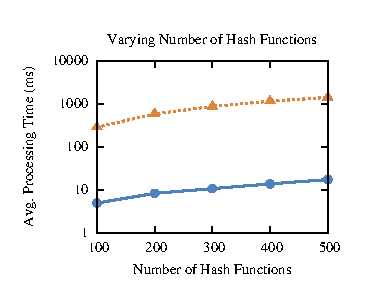
\includegraphics[width=0.45 \textwidth]{fig/vary_l.eps} 
\label{questVla}}
\quad
\subfigure[]{% i
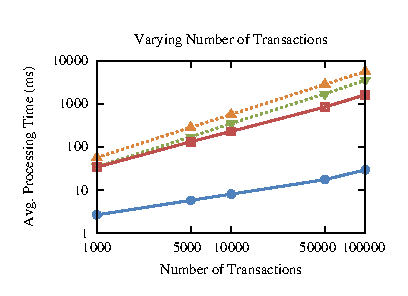
\includegraphics[width=0.45 \textwidth]{fig/vary_m.eps} 
\label{questVma}}

\caption{Average Processing Time on IBM Quest Data Set Using Jaccard Similarity}
\label{ibmTestsAvgEff}
\end{figure*}

\begin{figure*}[htb]
\centering
\subfigure[Large $|\Sigma|$]{% d
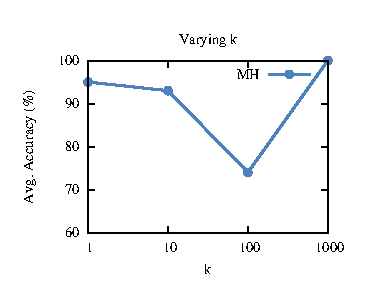
\includegraphics[width=0.45 \textwidth]{fig/acc_vary_k_large.eps} 
\label{questLLVkb}}
\quad
\subfigure[Small $|\Sigma|$]{% e
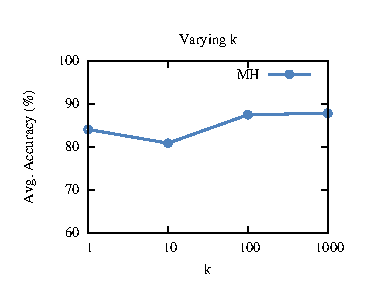
\includegraphics[width=0.45 \textwidth]{fig/acc_vary_k_small.eps} 
\label{questSLVkb}}
\quad
\subfigure[]{% f
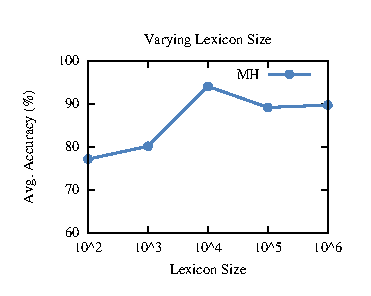
\includegraphics[width=0.45 \textwidth]{fig/acc_vary_lexicon.eps} 
\label{questVsigmab}}
\quad
\subfigure[]{% j
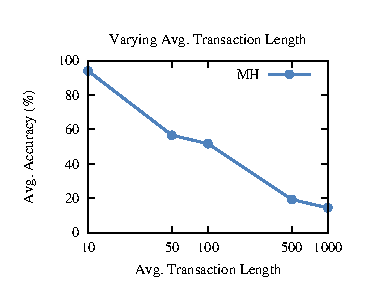
\includegraphics[width=0.45 \textwidth]{fig/acc_vary_tlen.eps} 
\label{questVnb}}
\quad
\subfigure[]{% k
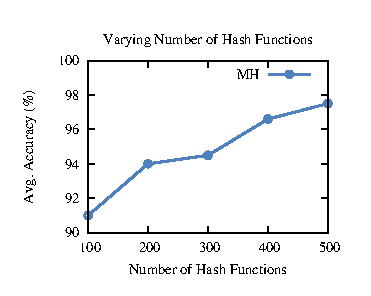
\includegraphics[width=0.45 \textwidth]{fig/acc_vary_l.eps} 
\label{questVlb}}
\quad
\subfigure[]{% l
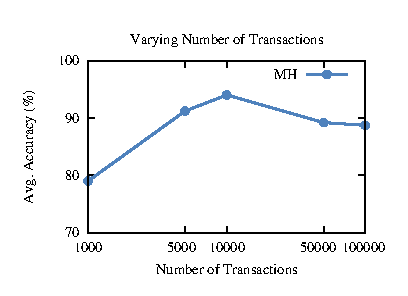
\includegraphics[width=0.45 \textwidth]{fig/acc_vary_m.eps} 
\label{questVmb}}
\caption{Average Accuracy of Hashing-based Method on IBM Quest Data Set Using Jaccard Similarity}
\label{ibmTestsAvgAcc}
\end{figure*}


\begin{figure*}[htb]
\centering
\subfigure[Large $|\Sigma|$]{% g
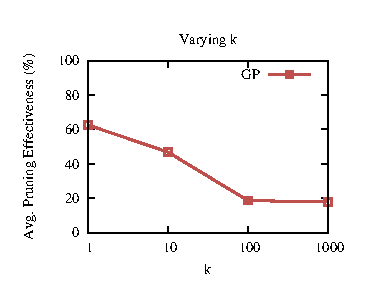
\includegraphics[width=0.45 \textwidth]{fig/preff_vary_k_large.eps} 
\label{questVkPreffL}}
\quad
\subfigure[Small $|\Sigma|$]{% h
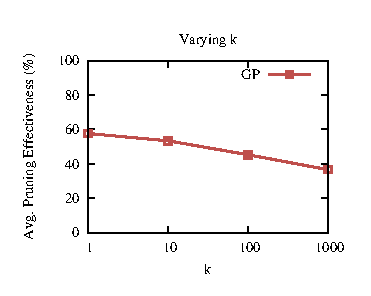
\includegraphics[width=0.45 \textwidth]{fig/preff_vary_k_small.eps} 
\label{questVkPreffS}}
\quad
\subfigure[]{% k
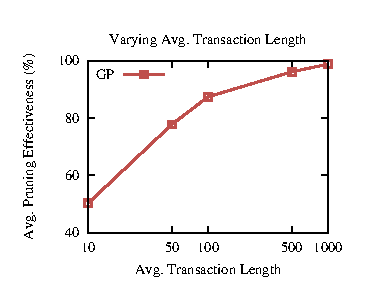
\includegraphics[width=0.45 \textwidth]{fig/preff_vary_tlen.eps} 
\label{questVnPreff}}
\quad
\subfigure[]{% j
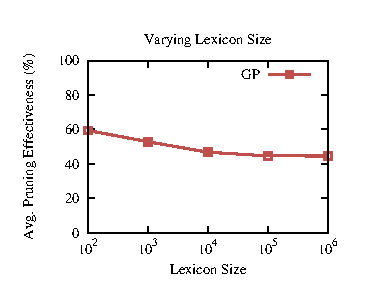
\includegraphics[width=0.45 \textwidth]{fig/preff_vary_lexicon.eps} 
\label{questVsigmaPreff}}
\quad
\raggedright
\subfigure[]{% i
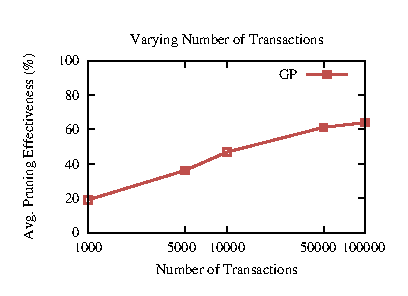
\includegraphics[width=0.45 \textwidth]{fig/preff_vary_m.eps} 
\label{questVmPreff}}
\caption{Pruning Effectiveness of GP on IBM Quest Data Set Using Jaccard Similarity}
\label{ibmTestsP3}
\end{figure*}


%Let us denote Algorithm~\ref{minHashBasic} as ``MHB'', which can be regarded as the baseline for hash-based algorithms. Algorithm~\ref{minHashInd} is named as ``MHI". Our first pruning-based algorithm is denoted as ``GP". 
To generate synthetic datasets using the IBM Quest data generator, we set parameters for $n$, $|\Sigma|$, and $m$. The synthetic query stream is generated by concatenating random objects whose lengths are between $0.8\bar{n}$ to $1.2\bar{n}$, where $\bar{n}$ is the average object length of the data set. In reality, the distribution of the elements in the stream would not change much in a very short time period. For example, on a Q\&A forum, some hot topics and its related ones may be discussed heavily for an hour before moving to the next groups of hot topics. In terms of average querying time, comparing to the real scenario, the performance of our algorithms using the generated query stream may be slower. It is because in our way of generating the stream, the transit from one topic to another is relatively faster than the typical real case.

We use the variable controlling method to conduct our experiments. The values of controlled variables along with the corresponding figures for each test are shown in Table~\ref{defaultVal}. In each variable controlled test, we compare the performance of GP and MHI, on the average querying time with two baseline methods, namely, BFM and MHB. BFM is a brute-force method that computes the exact similarity scores for every object with respect to a query. MHB is a baseline method based on MinHash technique but without indexing structures. To better illustrate how our upper bounds derived in Chapter~\ref{ch:pruning} can be used to prune unpromising objects, we define the pruning effectiveness of an update in Definition~\ref{preff-def}. In our experiments, we report the average pruning effectiveness of hundreds of updates. 

\begin{definition}[Pruning Effectiveness of Pruning-based Method]\label{preff-def}
Suppose we have $m$ objects in total and we compute the exact similarity scores for $m^*$ objects during an update. The pruning effectiveness of this update is $1 - \frac{m^*}{m}$. 
\end{definition}

The \emph{accuracy} in our context is defined in Definition~\ref{acc-methods}. The pruning algorithm GP always reports the exact query results, which has $100\%$ accuracy. However, since the MinHash-based methods compute similarity scores approximately, MHB and MHI give estimated answers to the top-$k$ query. We report the average accuracy of MinHash methods in Figure~\ref{ibmTestsAvgAcc}. 

\begin{definition}[Accuracy of a Method]\label{acc-methods}
Suppose the exact top-$k$ list regarding query $q_t$ is $top_k^{e}$ and the $k$-th best object is denoted as $o_{r_k}^e$. Given a method $A$ that returns a top-$k$ list, $top_k^A$, regarding query $q_t$, the accuracy of method $A$ is the proportion of objects in $top_k^A$ whose exact similarity scores regarding $q_t$ is no smaller than the $k$-th best similarity score in $top_k^{e}$. More formally, $acc_A$, the accuracy of method $A$ for $q_t$ is defined as $$acc_A = \frac{|\{o|o \in top_k^A \land sim(o, q_t)\geq sim(o_{r_k}^e, q_t)\}|}{k}\text{.}$$
\end{definition}

\begin{table}[t]
\caption{Values of Controlled Variables for Tests on Jaccard Similarity}  
\label{defaultVal} 
%\setlength{\tabcolsep}{0.5\tabcolsep}
\begin{center}%\resizebox{70mm}{!}
{
    \begin{tabular}{ |c|c|c|c|c|c|c|}
    \hline
    Test  & $k$ & $n$ & $|\Sigma|$ & $l$& $m$ &Figures\\ \hline
    Synthetic Data (Vary $k$) & n/a  &  $10$ & $10,000$  & $200$ & $10,000$  & Fig.~\ref{questLLVka}, \ref{questLLVkb}\\ \hline
    Synthetic Data (Vary $k$) & n/a &  $10$ &  $20$ & $200$ & $10,000$ & Fig.~\ref{questSLVka}, \ref{questSLVkb}\\ \hline
    Synthetic Data (Vary $|\Sigma|$) & $10$ &  $10$ &  n/a & $200$ & $10,000$  & Fig.~\ref{questVsigmaa}, \ref{questVsigmab}\\ \hline
    Synthetic Data (Vary $n$) & $10$ &  n/a &  $10,000$ & $200$ & $10,000$  & Fig.~\ref{questVna}, \ref{questVnb}\\ \hline
    Synthetic Data (Vary $l$) & $10$ &  $10$ &  $10,000$ & n/a & $10,000$  & Fig.~\ref{questVla}, \ref{questVlb}\\ \hline
    Synthetic Data (Vary $m$) & $10$ &  $10$ & $10,000$ & $200$ &  n/a   & Fig.~\ref{questVma}, \ref{questVmb}\\ \hline
    Market Basket (Vary $l$) & $10$ &  $10$ & $16,470$ & n/a &  $88,162$   & Fig.~\ref{mbdsVlTime}, \ref{mbdsVlAcc}\\ \hline
    Market Basket (Vary $k$) & n/a &  $10$ & $16,470$ & $200$ &  $88,162$   & Fig.~\ref{mbdsVkTime}, \ref{mbdsVkAcc}\\ \hline
    Click Stream (Vary $l$) & $10$ &  $5$ & $17$ & n/a &  $31,790$   & Fig.~\ref{msnbcVlTime}, \ref{msnbcVlAcc}\\ \hline
    Click Stream (Vary $k$) & n/a &  $5$ & $17$ & $50$ &  $31,790$   & Fig.~\ref{msnbcVkTime}, \ref{msnbcVkAcc}\\ \hline
    \end{tabular}}
\end{center}
%\setlength{\tabcolsep}{2\tabcolsep}
\end{table}

\subsection{Efficiency}    
The average querying time of the four methods when $k$ varies is shown in Figures~\ref{questLLVka} and \ref{questSLVka} for two synthetic data sets with large lexicon ($10^4$) and small lexicon ($20$), respectively. We can observe that in both cases, the two baseline methods almost have no change in average processing time and MHI that uses $200$ hash functions outperforms the other three methods greatly. The pruning effectiveness of GP is shown in Figure~\ref{questVkPreffL} and Figure~\ref{questVkPreffS} when the lexicon size is set to $10^4$ and $20$, respectively. GP's pruning power drops gradually because the similarity score of the $k$-th best object in the top-$k$ result tends to decrease when $k$ increases. Given other parameters fixed, the similarity score of the $k$-th best object in the result with respect to queries would be smaller. Thus, the pruning effectiveness generally is weaker in the case of larger lexicon size. 

Figure~\ref{questVsigmaa} provides a better illustration of the trends of different methods when the lexicon size changes. When the lexicon size increases by orders of magnitude, we can see that the pruning effectiveness drops from $59.4\%$ to $44.5\%$ gradually. Thus, the average processing time of GP increases. The average running time of MHB and BFM does not have obvious change with respect to lexicon size. However, the average running time of MHI first decreases and then increases. When the lexicon size is small, the length of each inverted list is relatively large. Thus, a change in MinHash value of the query may result in many updates in the estimated similarity scores. When lexicon size becomes very large, though the size of each inverted list is small, the number of unmatched MinHash values between the MinHash lists of the previous query and the new query increases, which results in more queries on the inverted indices. 

We also examine how the average query answering time changes with respect to average object length. The results on efficiency and pruning effectiveness are shown in Figures~\ref{questVna}, and~\ref{questVnPreff}. The average processing time of BFM increases linearly while the performance of MHB does not have obvious change with respect to average object length. It is because we have transformed the transctions of varied length into MinHash signatures of the same length. However, the average processing time of MHI first decreases slightly and then increases. When the average object length becomes larger, the size of each inverted list would be larger, which results in longer processing time. When the average object length increases, the pruning effectiveness of GP increases dramatically, from $46.8\%$ to $97.2\%$. However, its average running time still increases slightly, since there is an increase in computing exact similarity scores for larger sets in the verification phase.   
% reaches the minimum when the average transaction length is $10$.
% Done - Add: analyze MHI 

The results with respect to the number of hash functions is shown in Figure~\ref{questVla}.  The average processing time of MHB and MHI both increases linearly with the number of hash functions, which is in accordance with the analysis of our algorithms.  The scalability of three methods is shown in Figure~\ref{questVma}.  All the methods increases linearly as the number of object increases.  The pruning power of GP increases from $19.1\%$ to $64.0\%$ when the number of objects increases from $10^3$ to $10^5$, which is shown in Figure~\ref{questVmPreff}.   
% Done - Add: describe scalability 

\subsection{Accuracy}
We also test the accuracy of the MinHash-based algorithms. By our definition, the accuracy of the two MinHash-based algorithms are the same according to the same set of hash functions. We denote the MinHash methods by MH in the figures that report accuracy. The accuracy can be affected by two factors, the number of hash functions used and the intrinsic characteristics of our data set such as the distribution of similarity scores among objects. 
% For example, if there are many objects with close similarity scores to those of objects in the exact top-$k$ list, then the accuracy tends to be lower. 

In general, we can achieve an accuracy ranging from $70\%$ to $98\%$ when $200$ hash functions are used. Figures~\ref{questLLVkb} and~\ref{questSLVkb} show the change in accuracy when $k$ increases for data sets with large lexicon and small lexicon, respectively. In the case where lexicon size is $10^4$, the accuracy first decreases and then increases. The smallest average accuracy rate is achieved when $k = 10^2$. When $k$ is very large, say $10^3$, the $k$-th best similarity score would become $0$, which is the reason why the accuracy increases to $100\%$ when $k$ is $10^3$. This issue does not occur in the case of small lexicon. When lexicon size is $20$, we can achieve accuracy in the range of $80\%$ to $88\%$. The average accuracy first decreases and then increases, and the smallest average accuracy rate is achieved when $k = 10$.   

%%% test on retail.txt %%%
\begin{figure*}[htb]
\centering
\subfigure{% a
\label{legend}

\includegraphics[width=1\textwidth]{fig/legend_efficiency.eps}}
\quad
\setcounter{subfigure}{0}
\subfigure[]{% i
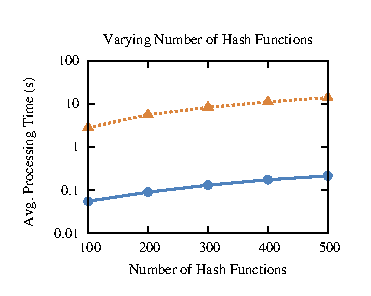
\includegraphics[width=0.45 \textwidth]{fig/rmarket_vary_l.eps} 
\label{mbdsVlTime}}
\quad
\subfigure[]{% j
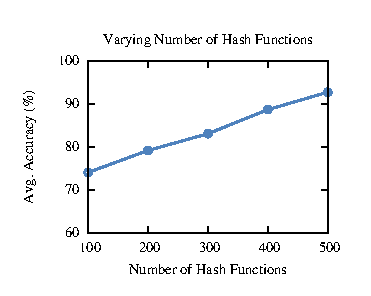
\includegraphics[width=0.45 \textwidth]{fig/rmarket_acc_vary_l.eps} 
\label{mbdsVlAcc}}
\quad
\subfigure[]{% g
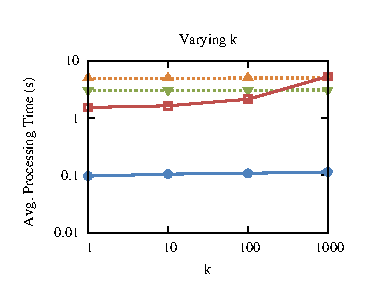
\includegraphics[width=0.45 \textwidth]{fig/rmarket_vary_k.eps} 
\label{mbdsVkTime}}
\quad
\subfigure[]{% h
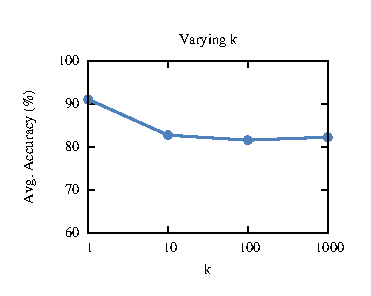
\includegraphics[width=0.45 \textwidth]{fig/rmarket_acc_vary_k.eps} 
\label{mbdsVkAcc}}
\quad
\raggedright
\subfigure[]{% i
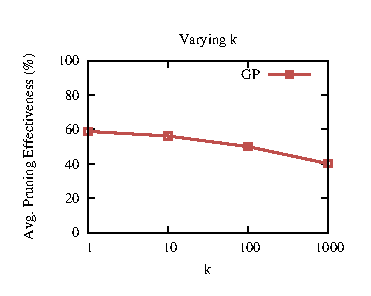
\includegraphics[width=0.45 \textwidth]{fig/rmarket_preff_vary_k.eps} 
\label{mbdsVkPreff}}
\caption{Results on Market Basket Dataset Using Jaccard Similarity}
\label{mbData}
\end{figure*}


The average accuracy increases quickly and then decreases slightly when the lexicon size increases, which is shown in Figure~\ref{questVsigmab}.  The highest accuracy is achieved when lexicon size is $10^4$.  In Figure~\ref{questVnb}, when the average object length increases from $10$ to $10^3$, the accuracy drops drastically from $94\%$ to $14.4\%$.  The reason is apparent.  More hash functions are needed to achieve the same level of accuracy when the set size gets larger. 
% Done - Correct: first sentence not consistent now

We also test the trend of accuracy when the number of hash functions and the number of objects increase.  The results are shown in Figures~\ref{questVlb} and \ref{questVmb}, respectively.  When more hash functions are used, the estimated Jaccard similarity is closer to the exact score, thus lead to higher accuracy.  As shown in Figure~\ref{questVlb}, we can see that the result follows this trend and we can achieve average accuracy rate ranging from $91\%$ to $97.5\%$.  Figure~\ref{questVmb} suggests that the average accuracy first increases and then decreases when the number of objects increases. The highest accuracy is achieved when $m = 10^4$.  

%%%%%% Real Data Set %%%%%%
\section{Results on Real Data Sets}
\label{sec:real-data}

\begin {table}[t]
\caption {Real Data Sets Statistics}  
%\setlength{\tabcolsep}{0.5\tabcolsep}
\label{datasetStat} 
\begin{center}%\resizebox{70mm}{!}
{
    \begin{tabular}{ |c|c|c|c|}
    \hline
    Data Set  & Cardinality & Avg. Length & Lexicon Size \\ \hline
    Market Basket & 88,162 & 10.306 & 16,470 \\ \hline
    MSNBC & 31,790 & 5.3338 & 17 \\ \hline
    \end{tabular}}
\end{center}
%\setlength{\tabcolsep}{2\tabcolsep}
\end {table}

We conduct experimental studies on two real data sets: a retail market basket data set\footnote{\url{http://fimi.ua.ac.be/data/}} from an anonymous Belgian retail store and MSNBC, a data set of click-stream data. We use a subset of the MSNBC data set that removes the shortest sequences, with the link provided \footnote{\url{http://www.philippe-fournier-viger.com/spmf/}}. We then transform each sequence into set. There is a significant difference in lexicon size of the two real data sets. The market basket data set has $16,470$ distinct items while the MSNBC data set contains only $17$ distinct items. Table~\ref{datasetStat} shows the detailed statistics of the data sets. To generate the querying stream, we randomly concatenate objects in the data set whose size is between $0.8\bar{n}$ to $1.2\bar{n}$, where $\bar{n}$ is the average object length of the data set. For each data set, we compare the average processing time and the average accuracy when $k$ or $l$ varies, respectively. The results are shown in Figure~\ref{mbData} and \ref{csData}. 

The trends of the curves for the market basket data set is highly consistent with the results on the synthetic data sets. In Figure~\ref{mbdsVlTime} and \ref{mbdsVlAcc}, we show the trends of processing time and accuracy of the MinHash based methods when different number of hash functions is used.  The average processing time of MHB and MHI both increases linearly with the number of hash functions.  The performance of MHI is around $50$ to $65$ times faster than MHB.  The average accuracy increases steadily from $74\%$ to $93\%$ when the number of hash functions increases from $100$ to $500$.  To compare the average processing time of different methods, we choose the default number of hash functions as $200$.  The processing time of BFM, MHB, and MHI does not have obvious change and MHI always has the best performance.  The pruning power of GP decreases from $60\%$ to $40\%$ gradually when $k$ increases.  Therefore, the processing time of GP increases when $k$ increases.  The MinHash based algorithms can achieve accuracy over $80\%$ when $k$ is varied from $1$ to $1000$, which is shown in Figure~\ref{mbdsVkAcc}. 

The results for the click stream data set is shown in Figure~\ref{csData}.  Since the average length of the objects in this data set is only $5.33$, the MinHash based algorithms do not need many hash functions in order to achieve very high accuracy.  As shown in Figure~\ref{msnbcVlAcc}, the average accuracy is above $90\%$ when over $30$ hash functions are used.  To test the preformance when $k$ varies, we use $30$ hash functions. MHI is still the best method with respect to average query answering time, which can outperform the BFM by more than an order of magnitude. Comparing to the results on market basket data set, the average accuracy of MinHash-based methods is generally higher while the pruning effectiveness of GP is lower for the click stream data set.  
% Done - Add: discuss the special case       



%%% test on msnbcSubSet.txt %%%
\begin{figure*}[htb]
\centering
\subfigure{% a
\label{legend}

\includegraphics[width=1\textwidth]{fig/legend_efficiency.eps}}
\quad
\setcounter{subfigure}{0}
\subfigure[]{% i
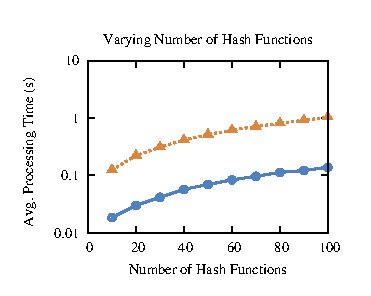
\includegraphics[width=0.45 \textwidth]{fig/rclicks_vary_l.eps} 
\label{msnbcVlTime}}
\quad
\subfigure[]{% j
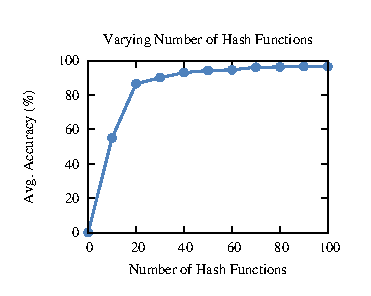
\includegraphics[width=0.45 \textwidth]{fig/rclicks_acc_vary_l.eps} 
\label{msnbcVlAcc}}
\quad
\subfigure[]{% g
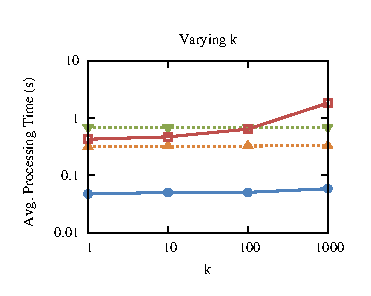
\includegraphics[width=0.45 \textwidth]{fig/rclicks_vary_k.eps}   
\label{msnbcVkTime}} 
\quad
\subfigure[]{% h 
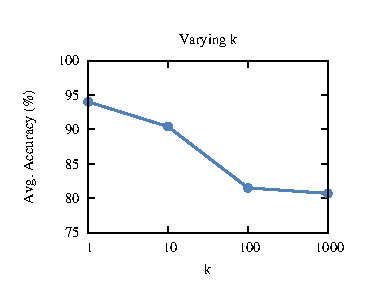
\includegraphics[width=0.45 \textwidth]{fig/rclicks_acc_vary_k.eps} 
\label{msnbcVkAcc}}
\quad
\raggedright
\subfigure[]{% i
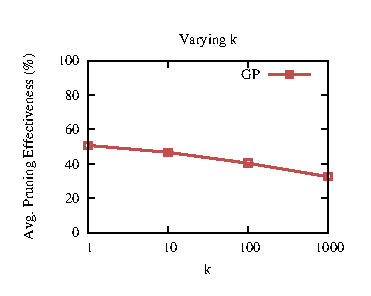
\includegraphics[width=0.45 \textwidth]{fig/rclicks_preff_vary_k.eps} 
\label{msnbcVkPreff}}

\caption{Results on Click Stream Dataset Using Jaccard Similarity}
\label{csData}
\end{figure*}

\section{Results on Other Similarity Measures}
\label{sec:other-measure}
In this section, we experiment on the performance of the bounds, derived in Section~\ref{sec:gen-sim}, for cosine similarity and edit similarity, using the click stream data set.  Since cosine similarity can be approximated using a random projection method~\cite{C02}, we can use the hashing-based framework for Jaccard similarity only with the signature generation phase changed. The random projection method chooses random hyperplanes defined by normal unit vectors and uses the signs of the dot products between the input vector and random hyperplanes as the signature for this vector. Given the signatures of two vectors generated by the same set of random hyperplanes, the percentage of matching bits in their signatures is proportional to the cosine distance between two vectors. Corresponding to MHB and MHI for Jaccard similarity, the hashing-based methods for cosine similarity are denoted as RPB and RPI. By default, we use $200$ random hyperplanes in our experiment.

The results for cosine similarity is shown in Figure~\ref{msnbcCos}.  The pruning effectiveness decreases from $86.0\%$ to $78.6\%$ when $k$ varies from $1$ to $1000$.  It is apparant since our similarity bound depends on the $k^{th}$ best score.  When $k$ increases, the $k^{th}$ best score decreases, thus less objects can be pruned. The average processing time increases when $k$ increases, which is in accordance with the trend of the pruning effectiveness. The pruning-based method has better performance, in terms of both querying time and accuracy, than the hashing-based method. We should notice that signatures constructed by random projection method only consist of $0$ and $1$. Since we use inverted indices in the same way as for Jaccard similarity, the number of objects in each inverted list would be very large. It can be the reason why the performance of the hashing-based algorithm becomes worse for cosine similarity.  

Figure~\ref{msnbcEd} shows the results for edit similarity on click stream data set. The trend is similar to that of cosine similarity and Jaccard similarity.  The algorithm can prune $64.8\%$ to $46.8\%$ objects when $k$ increases from $1$ to $100$.  Among the three distance measures, the bound for cosine similarity has the best pruning effectiveness; The bound for edit similarity comes second and the bound for Jaccard similarity is slightly worse than that of edit similarity.   
     
% Done - Add

\section{Summary of Results}
We conduct experiments to test the effectiveness and efficiency of our pruning-based method and hashing-based method. There are $5$ parameters that can affect the performance of our methods. We test our methods by varying one parameter in each test and compare the performance of our methods. 

Generally speaking, in terms of accuracy, the pruning-based method is an exact method while the hashing-based method can reach very good accuracy rate when a few hundreds of hash functions are used. For Jaccard similarity, the hashing-based method with good accuracy results can always achieve faster average querying time than the pruning-based method. However, for cosine similarity, the pruning method can achieve better performance than the hashing-based method. One reason is that the pruning effectiveness of cosine similarity is the highest among the three similarity measures in our experiments. The other reason is that the inverted indices can not reduce much work in updating the similarity scores since each inverted list can be very long with length equals to half of the number of transactions on average. 




% However, the accuracy rate is sensitive to the average number of items per object. For example, to achieve the same level of accuracy, we need $50$ hash functions when $n = 5$ while $100$ hash functions are required when $n = 10$. The performance of the pruning-based method is highly related to the similarity score between the evolving query and the $k^{th}$ best object in the top-$k$ result. If this score is very large while the similarity between the query and each object that are not currently in the top-$k$ result is very small, then we only need to compute a tiny portion of exact similarity scores in each update. 



% Let us consider an extreme case. If only a few number (close to $k$) of objects are very similar to the query and the other objects are very different, then we only need to compute a tiny portion of exact similarity scores in each update.  

%%% test on msnbcSubSet.txt for cosine sim %%%
%\vspace{-5 mm}
\begin{figure*}[htb]
\centering
\subfigure{% a
\label{legend}

\includegraphics[width=1\textwidth]{fig/legend_efficiency_rp.eps}}
\vspace{-5 mm}
\quad
\setcounter{subfigure}{0}
\subfigure[]{% d
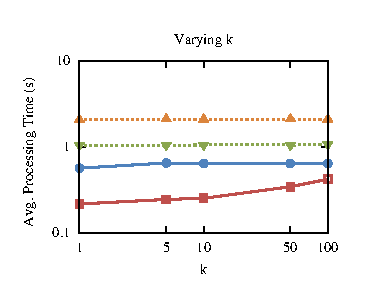
\includegraphics[width=0.445 \textwidth]{fig/rclicks_vary_k_cos.eps} 
%\label{msnbcVkCos}}
}
\quad
\subfigure[]{% e
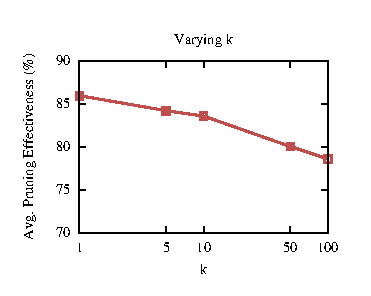
\includegraphics[width=0.445 \textwidth]{fig/rclicks_preff_vary_k_cos.eps} 
%\label{msnbcVkPreffCos}}
}
\quad 
\raggedright
\subfigure[]{% e
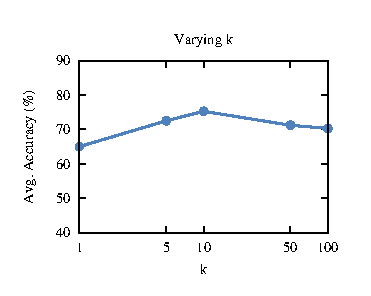
\includegraphics[width=0.445 \textwidth]{fig/rclicks_acc_vary_k_cos.eps} 
\label{msnbcVkAccCos}}
\vspace{-3mm}
\caption{Results on Click Stream Dataset Using Cosine Similarity}
\label{msnbcCos}
\end{figure*}
\vspace{-10 mm}
\begin{figure*}[htb]
\centering
\subfigure[]{% d
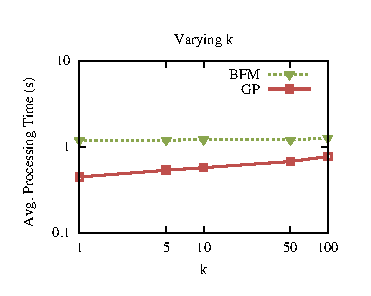
\includegraphics[width=0.445 \textwidth]{fig/rclicks_vary_k_ed.eps} 
\label{msnbcVkEd}}
\quad
\subfigure[]{% e
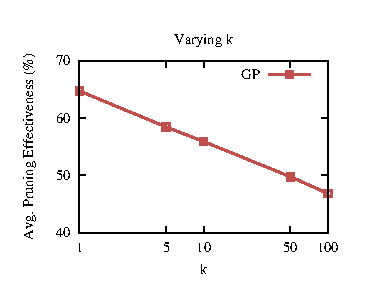
\includegraphics[width=0.445 \textwidth]{fig/rclicks_preff_vary_k_ed.eps} 
\label{msnbcVkPreffEd}}
\vspace{-3mm}
\caption{Results on Click Stream Dataset Using Edit Similarity}
\label{msnbcEd}
\end{figure*}

%\vspace{3 mm}


% Thus, the similarity score distribution in the data set and the number of similar objects we want to find. Although the   

% More specifically, there are $5$ parameters that can affect the performance of our methods, including the number of similar objects to select ($k$), lexicon size ($|\Sigma|$), average number of items per transaction ($n$), number of objects ($m$), and number of hash functions used ($l$). We test our methods by varying only one of the above parameters each time.   

    

%% Copyright 1998 Pepe Kubon
%%
%% `two.tex' --- 2nd chapter for thes-full.tex, thes-short-tex from
%%               the `csthesis' bundle
%%
%% You are allowed to distribute this file together with all files
%% mentioned in READ.ME.
%%
%% You are not allowed to modify its contents.
%%

%%%%%%%%%%%%%%%%%%%%%%%%%%%%%%%%%%%%%%%%%%%%%%%%%
%
%     Chapter 7  
%
%%%%%%%%%%%%%%%%%%%%%%%%%%%%%%%%%%%%%%%%%%%%%%%%

\chapter{Conclusions}
\label{ch:con}
%\section{Summary of the Thesis}

The skyline subspace problem is originally motivated by the problem of what distinguish one from its peers in social networks~\cite{lo2013distinguish}. In this thesis, we formulate the social network into a graph with labels and consider the distances between a person and the labels as the factors that distinguish the person from its peers. We propose a bottom-up algorithm to answer \emph{skyline subspace query} which is based on set enumeration and dominating candidate sets intersection. To tackle the problems of skyline subspaces on graph and the skyline subspaces on Euclidean space, we develop effective pruning methods to reduce the search space. 
We did empirical studies using both synthetic and real data sets to evaluate our approach. We generated the synthetic graph based on the Kronecker graph model and the real world datasets are from DBLP and YELP. The experimental results verify the efficiency of our algorithms.

As for future work, we can consider the following directions.  

\begin{itemize}
   
\item \textit{Using top-down set enumeration.} Our algorithm is based on bottom-up set enumeration. In bottom-up manner, we take the advantage of the property that if a target skyline subspace is found then we do not need to search for the subspaces that contain this subspace. For top-down approach, one of the advantage we can take is that if the query point is strictly dominated by some points in a certain subspace $\mathcal{A}$, then we do not need to check the subsets of the subspace $\mathcal{A}$ because we know that the query point cannot be a skyline point in those subspaces.

\item \textit{Further pruning method development in euclidean space.} There are many properties in euclidean space. In~\cite{sharifzadeh2006spatial}, Sharifzadeh et al. took the advantage of property of convex hull to reduce the size of skyline candidates. They also used the Voronoi diagram structure to index the graph. For future work, we can index the spatial points using Voronoi diagram instead of R-tree and applied pruning methods based on some geometry properties such as the property of convex hull.

\item \textit{Skyline subspace algorithm on other applications.} Finding the skyline subspaces on road networks and metric space is still an open problem. This topic is an interesting problem to be studied in the future.

\end{itemize}

















%%%%%%  bibliography
%%% Copyright 1998 Pepe Kubon
%%
%% `bibl.tex' --- bibliography for thes-full.tex, thes-short-tex from
%%                the `csthesis' bundle
%%
%% You are allowed to distribute this file together with all files
%% mentioned in READ.ME.
%%
%% You are not allowed to modify its contents.
%%

%%%%%%%%%%%%%%%%%%%%%%%%%%%%%%%%%%%%%%%%%%%%%%%%
%
%       Bibliography
%
%%%%%%%%%%%%%%%%%%%%%%%%%%%%%%%%%%%%%%%%%%%%%%%%

\nocite{*}     % everything cited automatically

\renewcommand{\baselinestretch}{\tighttextstretch} %% get smaller spacing
\normalsize

\bibliographystyle{plain}   %% dash under repeated name, von ignored
\addcontentsline{toc}{chapter}{Bibliography}
\typeout{Bibliography}
\bibliography{files/topk.bib}
\renewcommand{\baselinestretch}{\textstretch} %% get normal spacing
\normalsize


\addcontentsline{toc}{chapter}{Bibliography}
\typeout{Bibliography}
\bibliographystyle{abbrv}
\bibliography{topk}
\renewcommand{\baselinestretch}{\textstretch} %% get normal spacing
\normalsize


%%%  appendices, if any
%\begin{appendices}
%%% Copyright 1998 Pepe Kubon
%%
%% `appone.tex' --- 1st appendix for thes-full.tex, thes-short-tex from
%%                  the `csthesis' bundle
%%
%% You are allowed to distribute this file together with all files
%% mentioned in READ.ME.
%%
%% You are not allowed to modify its contents.
%%

%%%%%%%%%%%%%%%%%%%%%%%%%%%%%%%%%%%%%%%%%%%%%%%%%
%
%        Appendix 1
%
%%%%%%%%%%%%%%%%%%%%%%%%%%%%%%%%%%%%%%%%%%%%%%%%

\chapter{Appendices, sectioning}\label{app:spacing}
\index{appendices}\index{sectioning}

Appendices appear in the Contents table on the level of chapters and
numbered alphabetically starting from A. You can include normal
sectioning commands (notice the vertical spacing between different
levels):

\section{Section}\index{section}
A section is numbered and appears in the Contents.

\subsection{Subsection}\index{subsection}
Same holds for a subsection.

\subsubsection{Subsubsection}\index{subsubsection}
But not for other sectioning commands, unless you adjust the
\verb+secnumdepth+\index{secnumdepth@\texttt{secnumdepth} counter} and
\verb+tocdepth+\index{secnumdepth@\texttt{secnumdepth} counter}
counters to higher values (by default both are set to \texttt{2}).

\paragraph{Paragraph}\index{paragraph}
A paragraph is inlined.

\subparagraph{Subparagraph}\index{subparagraph}
A subparagraph is inlined and indented.




%%% Copyright 1998 Pepe Kubon
%%
%% `apptwo.tex' --- 2nd appendix for thes-full.tex from
%%                  the `csthesis' bundle
%%
%% You are allowed to distribute this file together with all files
%% mentioned in READ.ME.
%%
%% You are not allowed to modify its contents.
%%

%%%%%%%%%%%%%%%%%%%%%%%%%%%%%%%%%%%%%%%%%%%%%%%%%
%
%        Appendix 2
%
%%%%%%%%%%%%%%%%%%%%%%%%%%%%%%%%%%%%%%%%%%%%%%%%

\chapter{Illustrating Lists}\label{app:lists}
\index{formatting of Lists}

This appendix is present only in the full version of the thesis. It
illustrates in more detail the formatting of the Lists of Tables,%
\index{List of Tables}\index{List of Figures} Figures, etc. In
addition, it also illustrates the use of the ``other list'' facility
of \textsf{csthesis.sty}\index{csthesis.sty@\textsf{csthesis.sty}}.
Let us start with the latter.

\section{List of Programs}
\index{List of Programs}

In the preamble of \texttt{thes-full.tex}%
\index{thes-full.tex@\texttt{thes-full.tex}}, a new type of a floating
environment---\texttt{program}%
\index{program environment@\texttt{program} environment}---is defined,
together with the \verb+\otherlist+%
\index{otherlist@\texttt{\symbol{'134}otherlist}} command for
typesetting the List of Programs. The list is formatted in the same
way as the lists of Figures and Tables, and an appropriate entry is
added into Contents.

Because programs are defined here as floating environments, they are
typeset with the same (tighter) line-spacing%
\index{spacing in programs} as figures and tables:

\begin{program}[htbp]
  \begin{center}
    This shows that single line spacing\\
    is used inside programs.
    \caption{Example of the new \texttt{program} environment\label{prog1}}
  \end{center}
\end{program}
%
\vspace*{-.3in}
\begin{program}[htbp]
  \begin{center}
    A second example of a program environment.
    \caption{Second program\label{prog2}}
  \end{center}
\end{program}

\section{Formatting of Lists}

The tables (figures, programs, etc.) are organized and sorted by
chapters (appendices), with additional small vertical space separating
the chapter blocks. To illustrate this, I include two new tables here
(see List of Tables, etc., in the beginning of the thesis for the
result)\index{formatting of Lists}:

\begin{table}[htbp]
  \begin{center}
    To be silly or not to be silly\\
    \emph{that} is the question!
    \caption{First meaningless table in Appendix~\ref{app:lists}}
  \end{center}
\end{table}
%
\vspace*{-.3in}
\begin{table}[htbp]
  \begin{center}
    $F = nd^{2}$
    \caption{Second meaningless table in Appendix~\ref{app:lists}}
  \end{center}
\end{table}


%\end{appendices}


%%%%%%  index
%% Copyright 1998 Pepe Kubon
%%
%% `ind.tex' --- index for thes-full.tex from
%%               the `csthesis' bundle
%%
%% You are allowed to distribute this file together with all files
%% mentioned in READ.ME.
%%
%% You are not allowed to modify its contents.
%%

%%%%%%%%%%%%%%%%%%%%%%%%%%%%%%%%%%%%%%%%%%%%%%%%
%
%       Index
%
%%%%%%%%%%%%%%%%%%%%%%%%%%%%%%%%%%%%%%%%%%%%%%%%

\renewcommand{\baselinestretch}{\tighttextstretch} %% get smaller spacing
\normalsize

\addcontentsline{toc}{chapter}{Index}
\typeout{Index}
\printindex

\renewcommand{\baselinestretch}{\textstretch} %% get normal spacing
\normalsize



\end{document}







%%% Local Variables: 
%%% mode: latex
%%% TeX-master: t
%%% End: 
